%--------------- Personalize your document here ---------------

\author{Indra Yanto Simanihuruk} % Enter your name
%\newcommand{\studentID}{} % enter your student ID
\newcommand{\supervisorone}{Louis Owen} % Enter your supervisor's name
\newcommand{\supervisortwo}{}% Leave it empty or enter your second supervisor's name 
\newcommand{\department}{DATA SCIENCE BOOTCAMP BATCH 7}
\newcommand{\exam}{HOMEWORK DAY 16}

\title{Telco Customer Churn Analysis} %Enter the title of your report 
\date{December 2021} % insert a specific date	

%--------------------------------------------------------------

% This document was adapted from the
% TEMPLATE FOR PHYS250 WORKSHEET created by Alastair McLean
% URL: https://www.overleaf.com/latex/templates/phys250-worksheet-template/xxftvfhmwqdt

% Jefferson Silveira
% Email: 19jdls1@queensu.ca
% Last update: 09-Jun-2021
% If you have any questions or concerns, do not hesitate to contact me.
%--------------------------------------------------------------

\documentclass[a4paper,12pt]{article}
\usepackage[left=30mm,top=30mm,right=30mm,bottom=30mm]{geometry}
\usepackage{etoolbox} %required for cover page
\usepackage{booktabs}
\usepackage{pdflscape}
\usepackage[usestackEOL]{stackengine}
\usepackage[utf8]{inputenc}
\usepackage{bm}
\usepackage{graphicx}
\usepackage{subcaption}
\usepackage{amsmath}
\usepackage{amsfonts}
\usepackage{mathtools}
\usepackage{xcolor}
\usepackage{float}
\usepackage{hyperref}
\usepackage[capitalise]{cleveref}
\usepackage{enumitem,kantlipsum}
\usepackage{amssymb}
\usepackage[square,numbers,sort]{natbib}
\usepackage[ruled,vlined]{algorithm2e}
\usepackage{listings}
\usepackage{minted}
\usepackage{longtable}
\usemintedstyle{emacs}

\renewcommand{\listingscaption}{Algorithm}
\renewcommand{\listoflistingscaption}{List of Algorithms}


\bibliographystyle{unsrtnat}

\hypersetup{
	colorlinks,
	linkcolor={black},
	citecolor={blue!50!black},
	urlcolor={blue!80!black}
}

\linespread{1}

\newtheorem{theorem}{Theorem}[section]
\graphicspath{{figures/}}	

%----------------------------------TITLE PAGE -----------------------------------
\makeatletter
\def\maketitle{
	\begin{center}\leavevmode
		\normalfont
		
\includegraphics[width=0.35\columnwidth]{dibimbingid}
		\vskip 0.5cm   
		\textsc{\large \department}\\
		\vskip 1.5cm
		\rule{\linewidth}{0.2 mm} \\
		{\large \exam}\\[1 cm]
		{\huge \bfseries \@title \par}
		\vspace{1cm}
		\rule{\linewidth}{0.2 mm} \\[1.5 cm]
		
		\begin{minipage}[t]{0.45\textwidth}
			\begin{flushleft} \large
				\emph{Author:}\\
				\@author\\
				%Student ID: \studentID
			\end{flushleft}
		\end{minipage}
		\begin{minipage}[t]{0.45\textwidth}
			\begin{flushright} \large
				\ifdefempty{\supervisortwo}{\emph{Supervisor:\\}}{\emph{Supervisors:\\}}
				\supervisorone\\
				\ifdefempty{\supervisortwo}{}{\supervisortwo\\}
			\end{flushright}
		\end{minipage}
		\vfill
		{\Large \@date\par}
	\end{center}
	%\vfill
	%\null
	\cleardoublepage
}
\makeatother


%-------------------------------- ENDTITLE PAGE ----------------------------------

\begin{document}
	
	\pagenumbering{gobble}% Remove page numbers (and reset to 1)
	
	\maketitle
	
%	\begin{center}
%	\phantomsection
%	\pagenumbering{roman}
%	\addcontentsline{toc}{section}{Executive Summary}
%	\large{\textbf{Executive Summary}}
%	\end{center}
%sdasdas sdsa 
%	\newpage
	
	\tableofcontents
	\addcontentsline{toc}{section}{Contents}
	\newpage
	%\listoffigures
	%\newpage
	%\listoftables
	%\newpage
	%\listofalgorithms % List of algorithms in pseudocode format
	%\newpage
	%\listoflistings % List of algorithms in code format
	%\newpage
	
	
	% Arabic page numbers (and reset to 1)
	\pagenumbering{arabic}
	\setcounter{page}{1}
	% This is how you can organize your document
	\section{Introduction}
\subsection{Background}
	Telephone and Internet services are now considered essential in most aspects of human life. This leads to rapid and persistent growth in the telecom industries and makes customer loyalty one of the key aspects of surviving competitive market conditions. According to a study carried out by Bain \& Company \cite{bain}, the acquisition of new customers can cost the company 5 times more than what customer retaining will do. Moreover, it also states that increasing customer retention rates by 5\% can increase profits by 25\% at least.  
	
	
	Churn rate is one of the important metrics for customer retention study that indicates if customers stop doing business with the corresponding company. It surely has negative effect on company's profit and need to be minimized so the company can continue to run. The reason for this churn decision are usually a combination of some factors such as poor service quality, better competitor exists, high prices, and so on.
	
	The valuable basis to analyze this churn metric is none other than the data of customer itself. In this work, the data of certain telecom company will be studied to understand spesific customer who is likely to churn and the reasons behind that decision. Thus, the company can learn from it and come with reactive plans in the future. The dataset has also been pre-modified so it won't harm any customer's privacy.

\subsection{Data Source}
The customer base dataset used in this work is made available by IBM and downloaded from Kaggle \cite{kaggle}. It is related to an anonymous telecom company and contains 7043 customers data with 21 attributes where each row represents a customer and each column contains customer’s attributes. Overall, the dataset provides information about :
\begin{itemize}
	\item The target variable is Churn, indicates customers who left within the last month.
	\item Services that each customer signed up for, consist of phone service, multiple lines, internet, online security, online backup, device protection, tech support, and streaming TV and movies.
	\item The information about customer account consists of tenure, contract, payment method, paperless billing, monthly charges, and total charges.
	\item There are also gender, age range, partners, and dependents to give information about customer demographic.
\end{itemize}

The dataset will be analyzed using Google Collab (Python environment) \cite{indra}. This work used a few of libraries such as  pandas, NumPy, Matplotlib, seaborn, and plotnine.

\subsection{Business Objectives}
The analysis is carried out to answer this problem :
\begin{enumerate}
	\item Who are the customers more likely to churn and what are the probable reasons behind that decision?
	\item What actions can be taken to prevent them from leaving?
\end{enumerate}

	\section{Data Profiling and Cleansing}
\subsection{Data Profiling}

The dataset has 7043 rows and 21 columns which include informations about :
\begin{longtable}{p{0.25\textwidth}p{0.65\textwidth}}
\caption{Description of each column.}
\label{tab:columndesc}
\endfirsthead
\hline
Column & Description\\ \hline
customerID & Represents Unique Id Number of each customer (do not give any useful informations) \\
gender & Represents the customer gender \\
SeniorCitizen & Whether the customer is a senior citizen or not (1, 0) \\
Partner & Categorical data, identifies whether the customer has a partner or not (Yes, No)\\
Dependents & Whether the customer has dependents or not (Yes, No) \\
tenure & Number of months the customer has stayed with the company\\
PhoneService & Whether the customer has a phone service or not (Yes, No)\\
MultipleLines & Whether the customer has multiple lines or not (Yes, No, No phone service)\\
InternetService & Customer’s internet service provider (DSL, Fiber optic, No)\\
OnlineSecurity & Whether the customer has online security or not (Yes, No, No internet service)\\
OnlineBackup & Whether the customer has online backup or not (Yes, No, No internet service)\\
DeviceProtection & Whether the customer has device protection or not (Yes, No, No internet service)\\
TechSupport & Whether the customer has tech support or not (Yes, No, No internet service)\\
StreamingTV & Whether the customer has streaming TV or not (Yes, No, No internet service)\\
 StreamingMovies & Whether the customer has streaming movies or not (Yes, No, No internet service)\\
 Contract & The contract term of the customer (Month-to-month, One year, Two year)\\
 PaperlessBilling & Whether the customer has paperless billing or not (Yes, No)\\
 PaymentMethod & The customer’s payment method (Electronic check, Mailed check, Bank transfer/automatic, Credit card/automatic)\\
 MonthlyCharges & The amount charged to the customer monthly\\
TotalCharges & The total amount charged to the customer\\
 Churn &Target variable, define whether the customer churns or not (Yes or No)\\ \hline
\end{longtable}
One can clearly see from Table \ref{tab:columndesc} that most columns (17) are categorical variables except customerID, tenure, MontlyCharges, and TotalCharges. The customerID variable is feature that represents unique Id number of each customer (in total has 7043 unique values) hence it won't give any useful informations and will be dropped from analysis  meanwhile tenure, MonthlyCharges and TotalCharges are considered as numerical variables.



\subsection{Data Cleansing}
It's important to eliminate all missing values and anomalies from the data before it will be analyzed further. In this telco customer dataset, TotalCharges is the only column where a few of missing values are detected.
\begin{figure}[tbph]
	\centering
	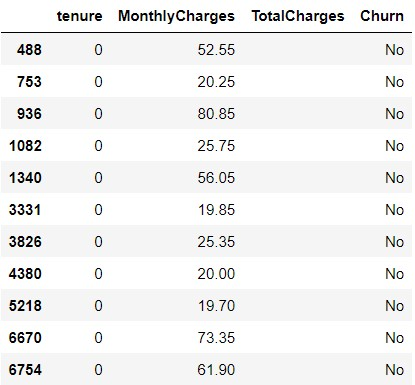
\includegraphics[width=0.6\linewidth]{figures/miss_values}
	\caption{All missing values detected in TotalCharges match 0 tenure period.}
	\label{fig:missvalues}
\end{figure}

There are in total 11 rows with missing value found in TotalCharges column and the reason behind these missing values is actually related to 0 tenure month (there are also 11 rows with 0 tenure). In addition, these rows with 0 period of tenure may emphasize the customer that has just signed up for the telecom service within the last month. Since they won't provide any useful information (the customers have just signed up) and the amount of rows are only 11, i.e 0.1\% of total rows, these rows will be eliminated and not included in the analysis.

Another thing one should be wary of before doing the analysis is the outlier.  An outlier is a value that deviates extremely from the rest observations within the sample data.  It may indicate bad and wrong observations or anomalies that need to be eliminated from the data. However, there are certain circumstances that outliers can reveal insights into special cases within the data that one may not otherwise notice. The best practice to detect the outlier is to use boxplot and it is shown in Figure \ref{fig:outlier1} that there is no outlier in the dataset.
\begin{figure}[tbph]
	\centering
	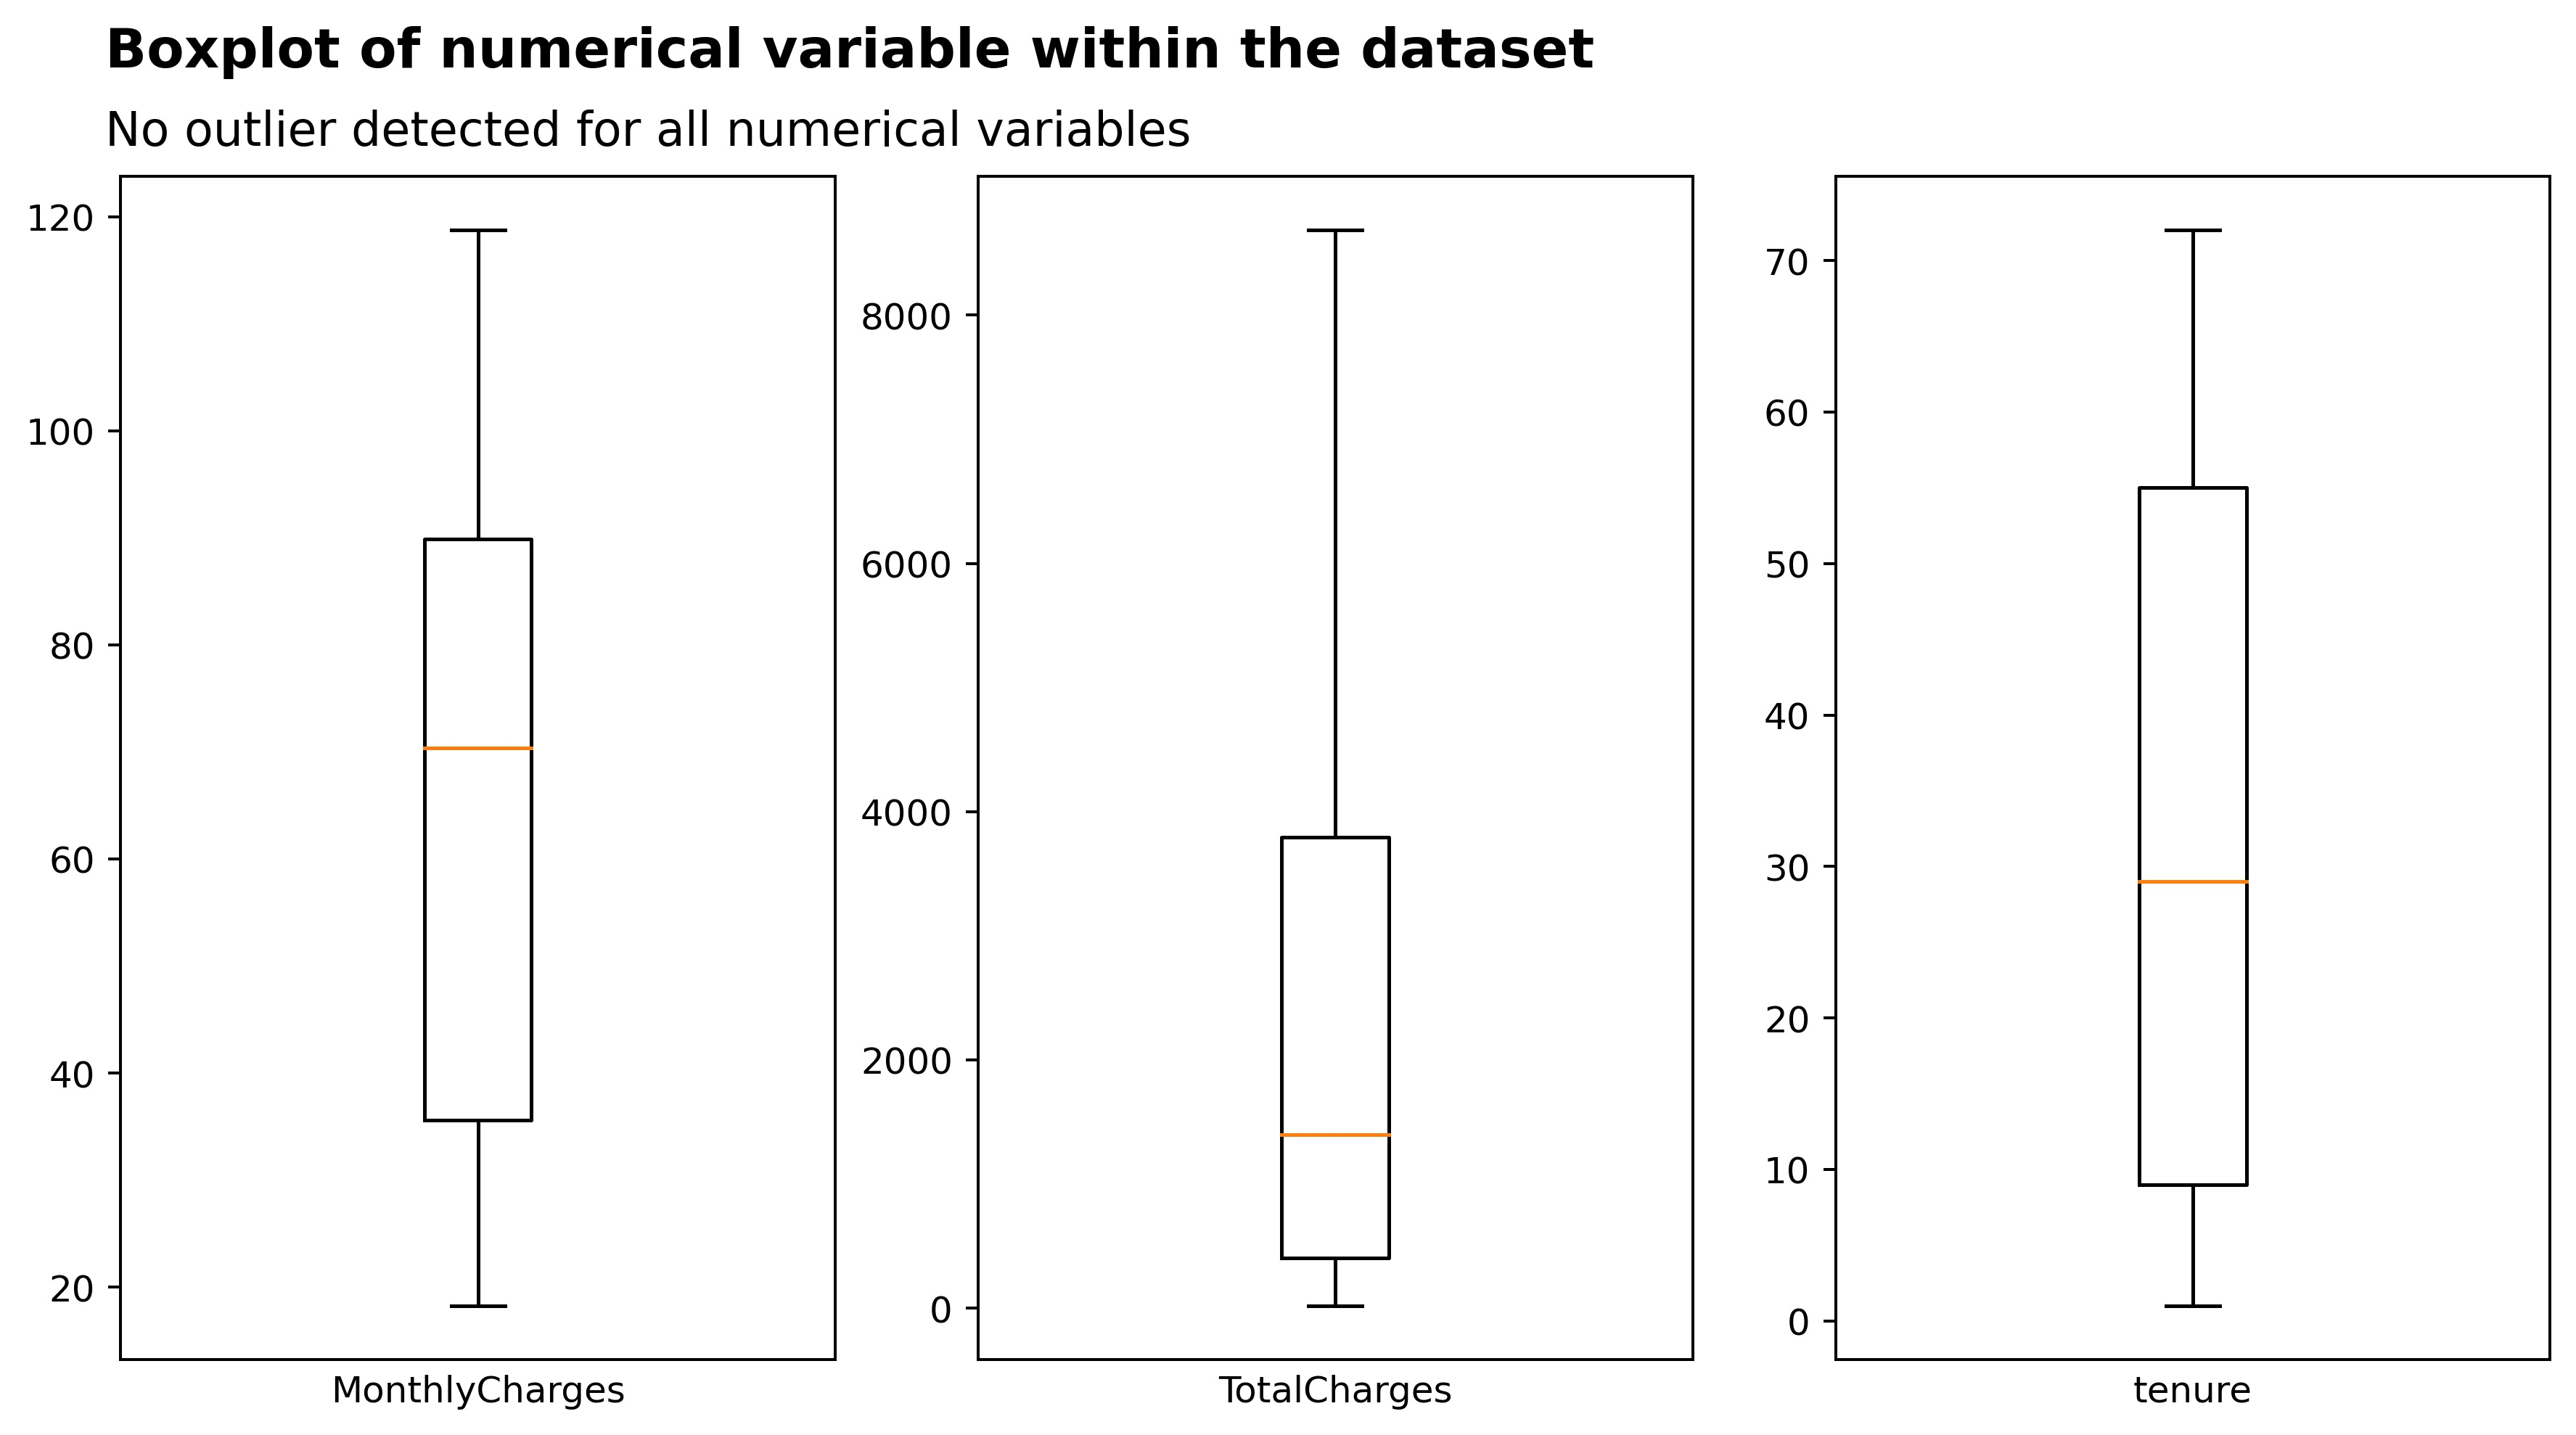
\includegraphics[width=1\linewidth]{figures/outlier1}
	\caption{No outlier found in the boxplots of MonthlyCharges, TotalCharges, and tenure.}
	\label{fig:outlier1}
\end{figure}


	\section{Exploratory Data Analysis}
\subsection{Univariate Analysis}

\begin{figure}[tbph]
	\centering
	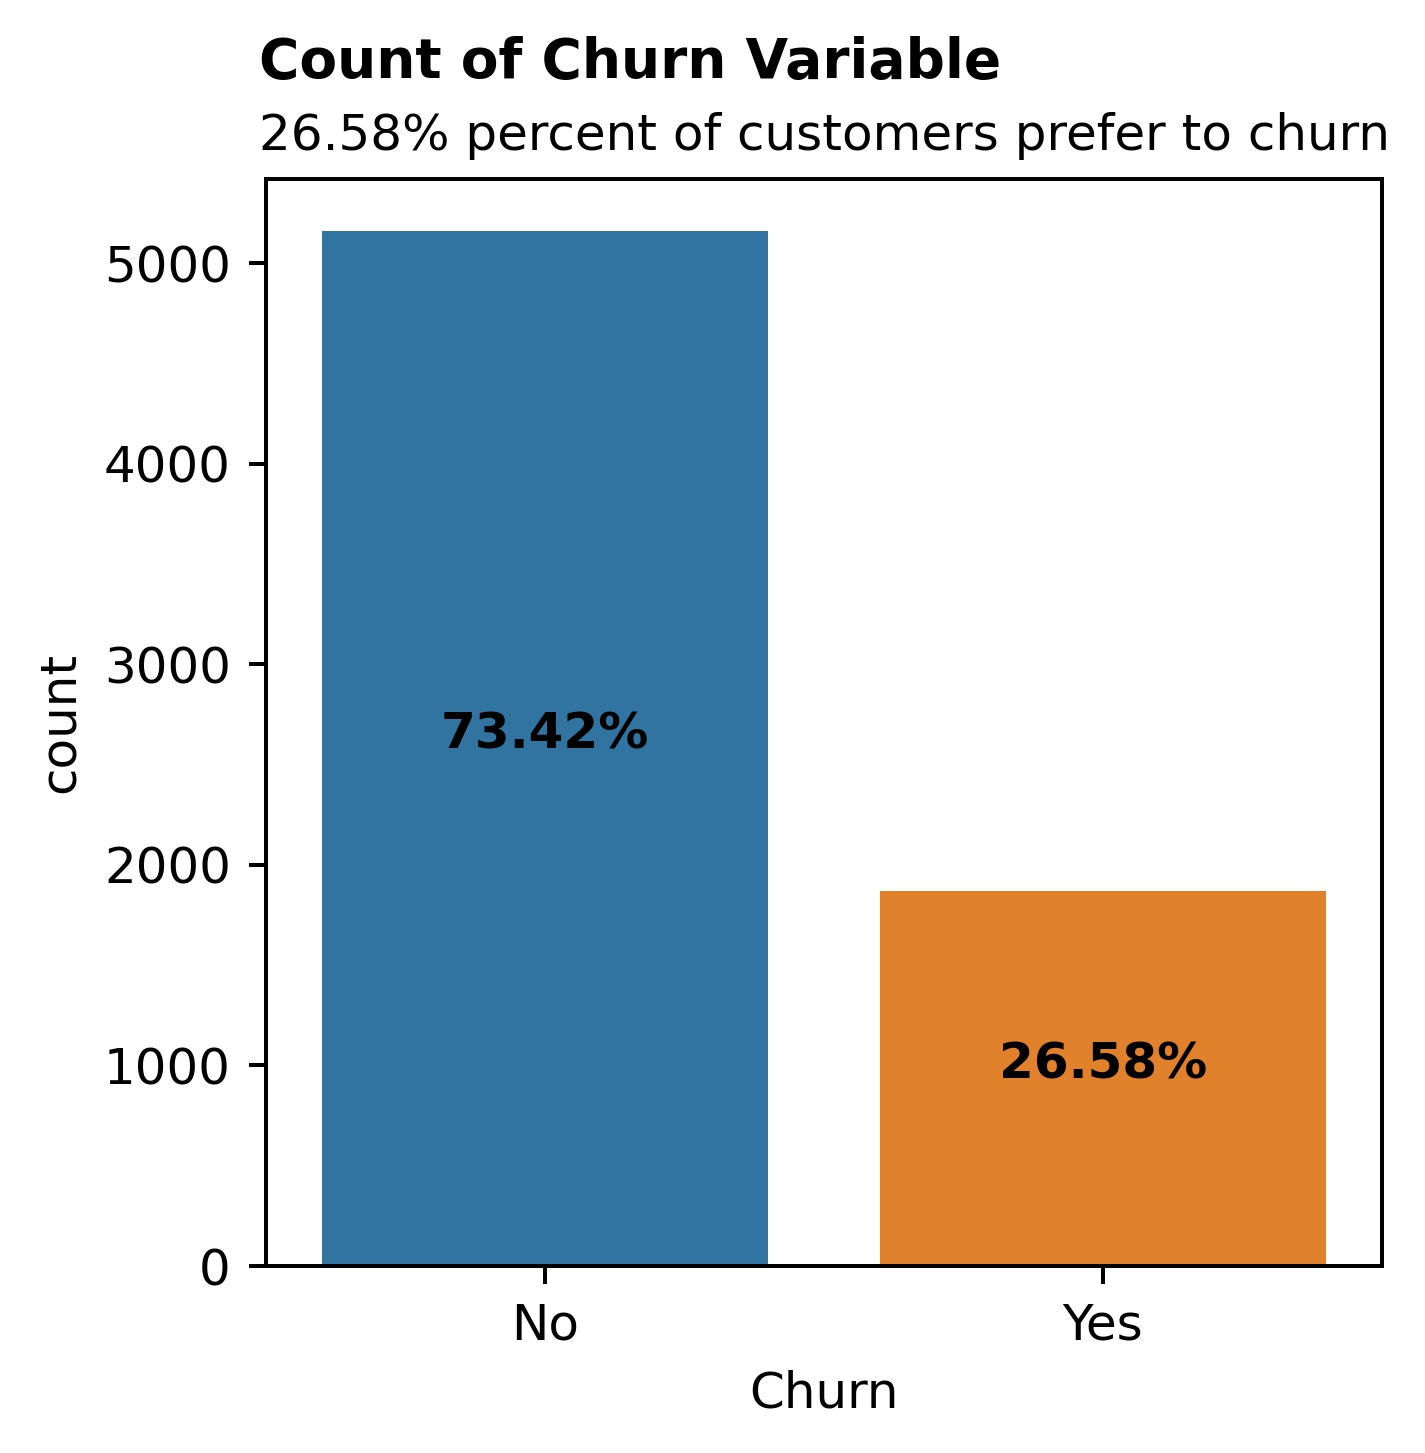
\includegraphics[width=0.5\linewidth]{figures/churn_univariate}
	\caption{Univariate analysis of Churn variable.}
	\label{fig:churn_univariate}
\end{figure}

In this univariate analysis, categorical variables will be viewed using a bar chart, whereas numerical variables will use the histogram. First, the analysis will be done for the target variables, Churn. From Figure \ref{fig:churn_univariate}, it can be seen that there is an imbalance for the target variable since it contains 5163 rows of No entries (73.42\%) and 1869 rows of Yes entries (26.58\%), indicates that the corresponding company has 26.57\% churn rate within the last month.
\begin{figure}[tbph]
	\centering
	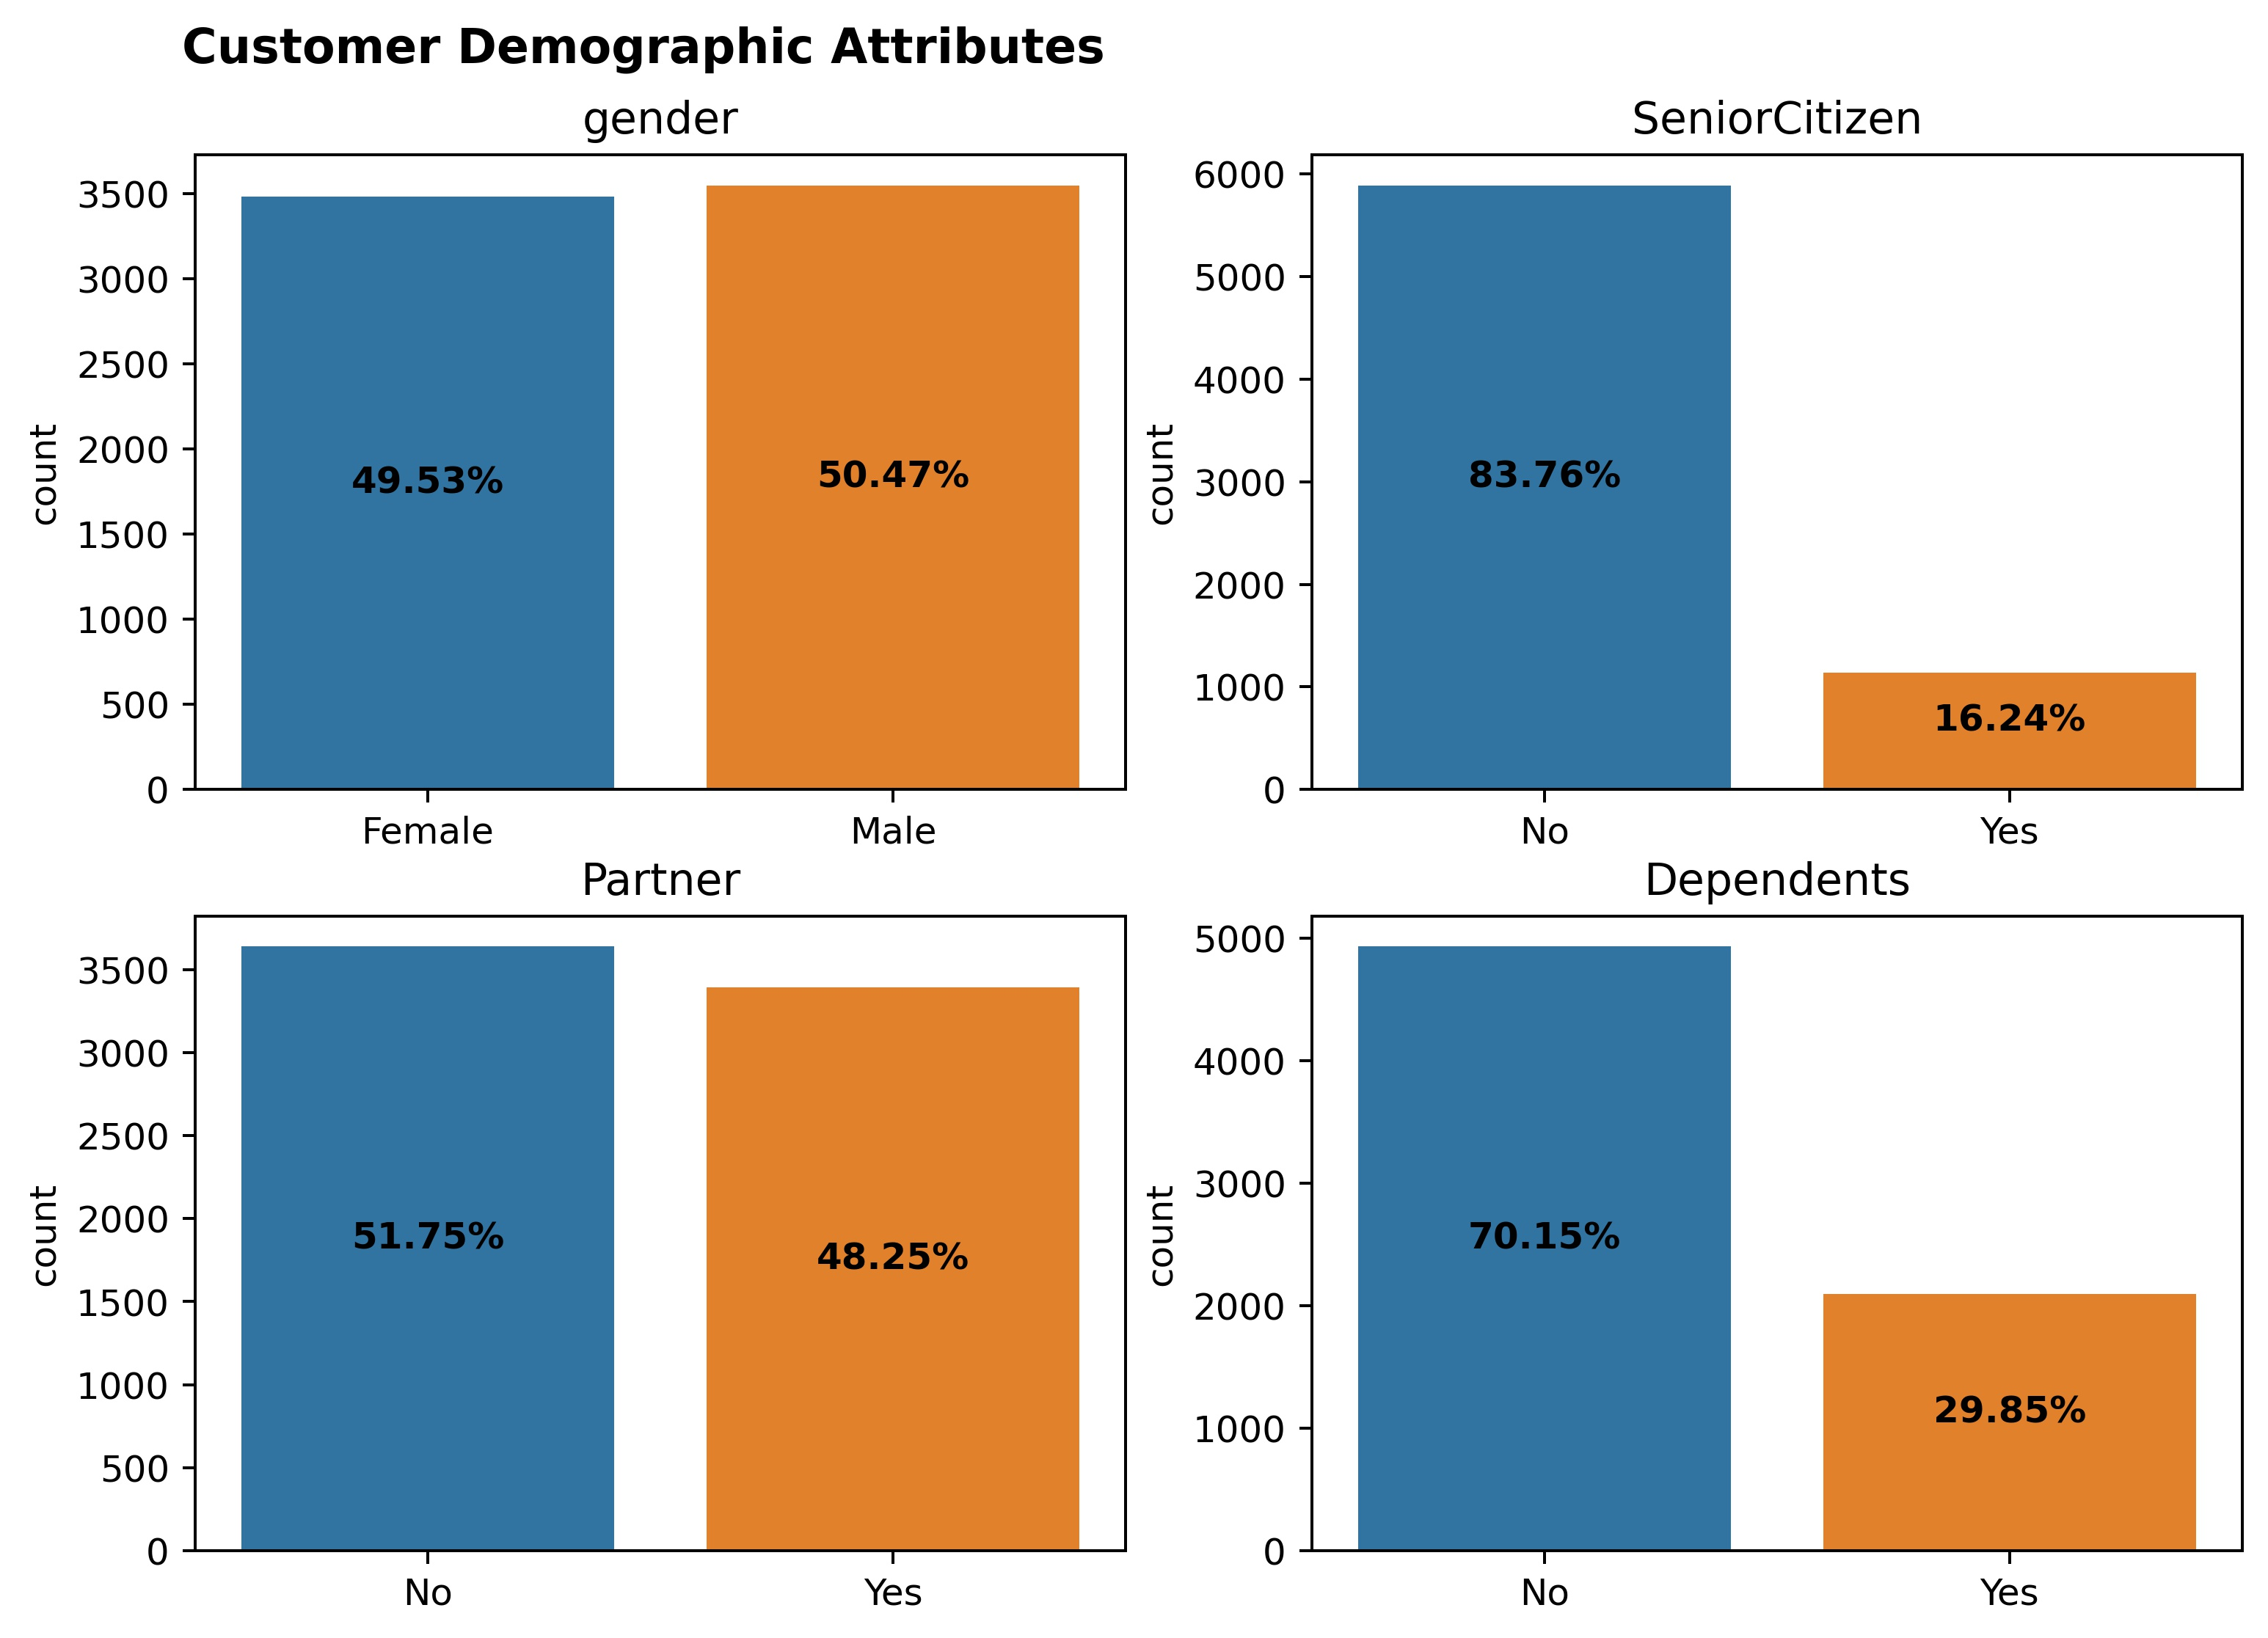
\includegraphics[width=1\linewidth]{figures/customer_demo}
	\caption{Univariate analysis of customer demographic attributes.}
	\label{fig:customer_demo}
\end{figure}

Next is the customer demographic attributes that consist of gender, Senior Citizen, Partner and Dependents. To analyze each variable uniformly, the binary integer value of Senior Citizen variable (1,0) will be converted into Yes or No beforehand.  For Figure \ref{fig:customer_demo} one can find that within the sample, the amount of each gender is approximately equal. The same applies to the Partner variable as the number of customers with or without a partner is also roughly similar. The distribution of imbalances can be seen by other features that around 16\% of customers are considered elderly and 30\% of customers have dependents.

\begin{figure}[tbph]
	\centering
	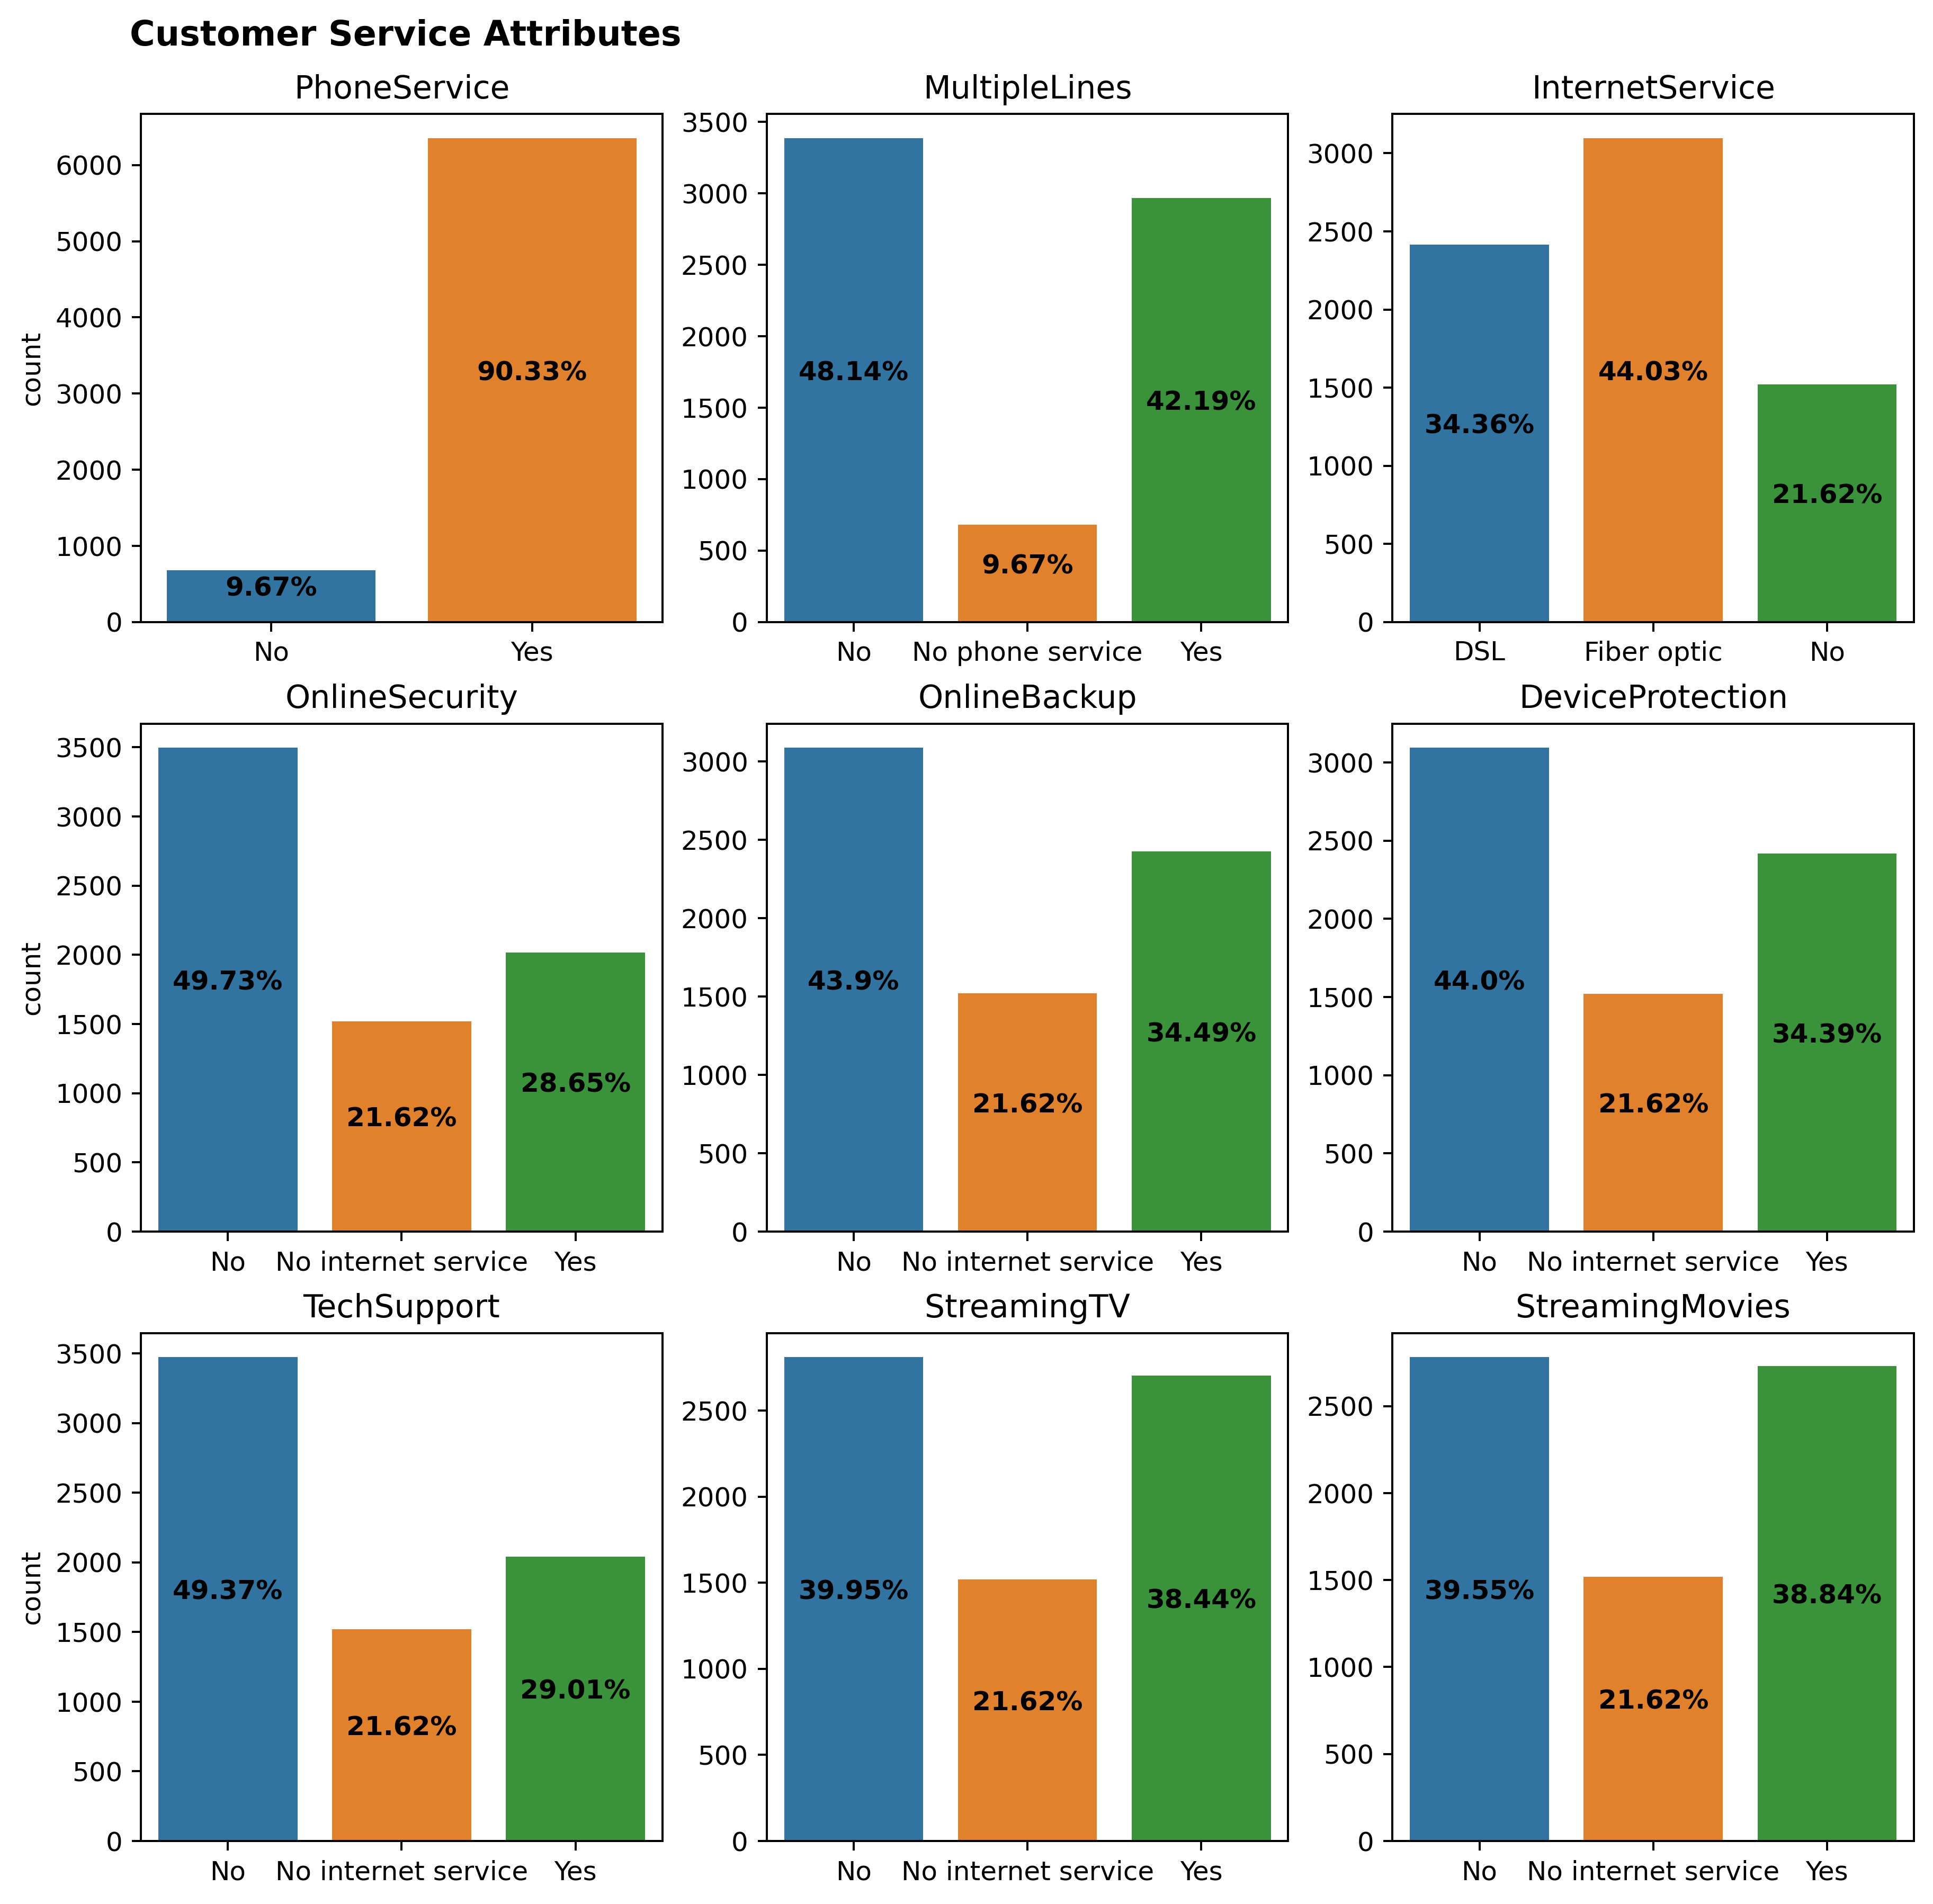
\includegraphics[width=1\linewidth]{figures/customer_service}
	\caption{Univariate analysis of customer service attributes.}
	\label{fig:customer_service}
\end{figure}

There are 9 variables that provide information about the services the customer signs up for. Figure \ref{fig:customer_service} shows that approximately 90\% of customers subscribe to telephone service and 42\% also subscribe to multi-line service as well. It also shows that the majority of customers also subscribe to an Internet service with 44\% of customers prefer the type of fiber optic service and 34\% choose DSL. It is apparent that most customers who use the Internet service prefer not to use some additional Internet services such as OnlineSecurity, OnlineBackup, DeviceProtection and TechSupport. However, the same thing does not apply to the streaming service since the number of customers using or not using the service is similar. This also means that the streaming service is the most popular among the additional internet services.

\begin{figure}[t]
	\centering
	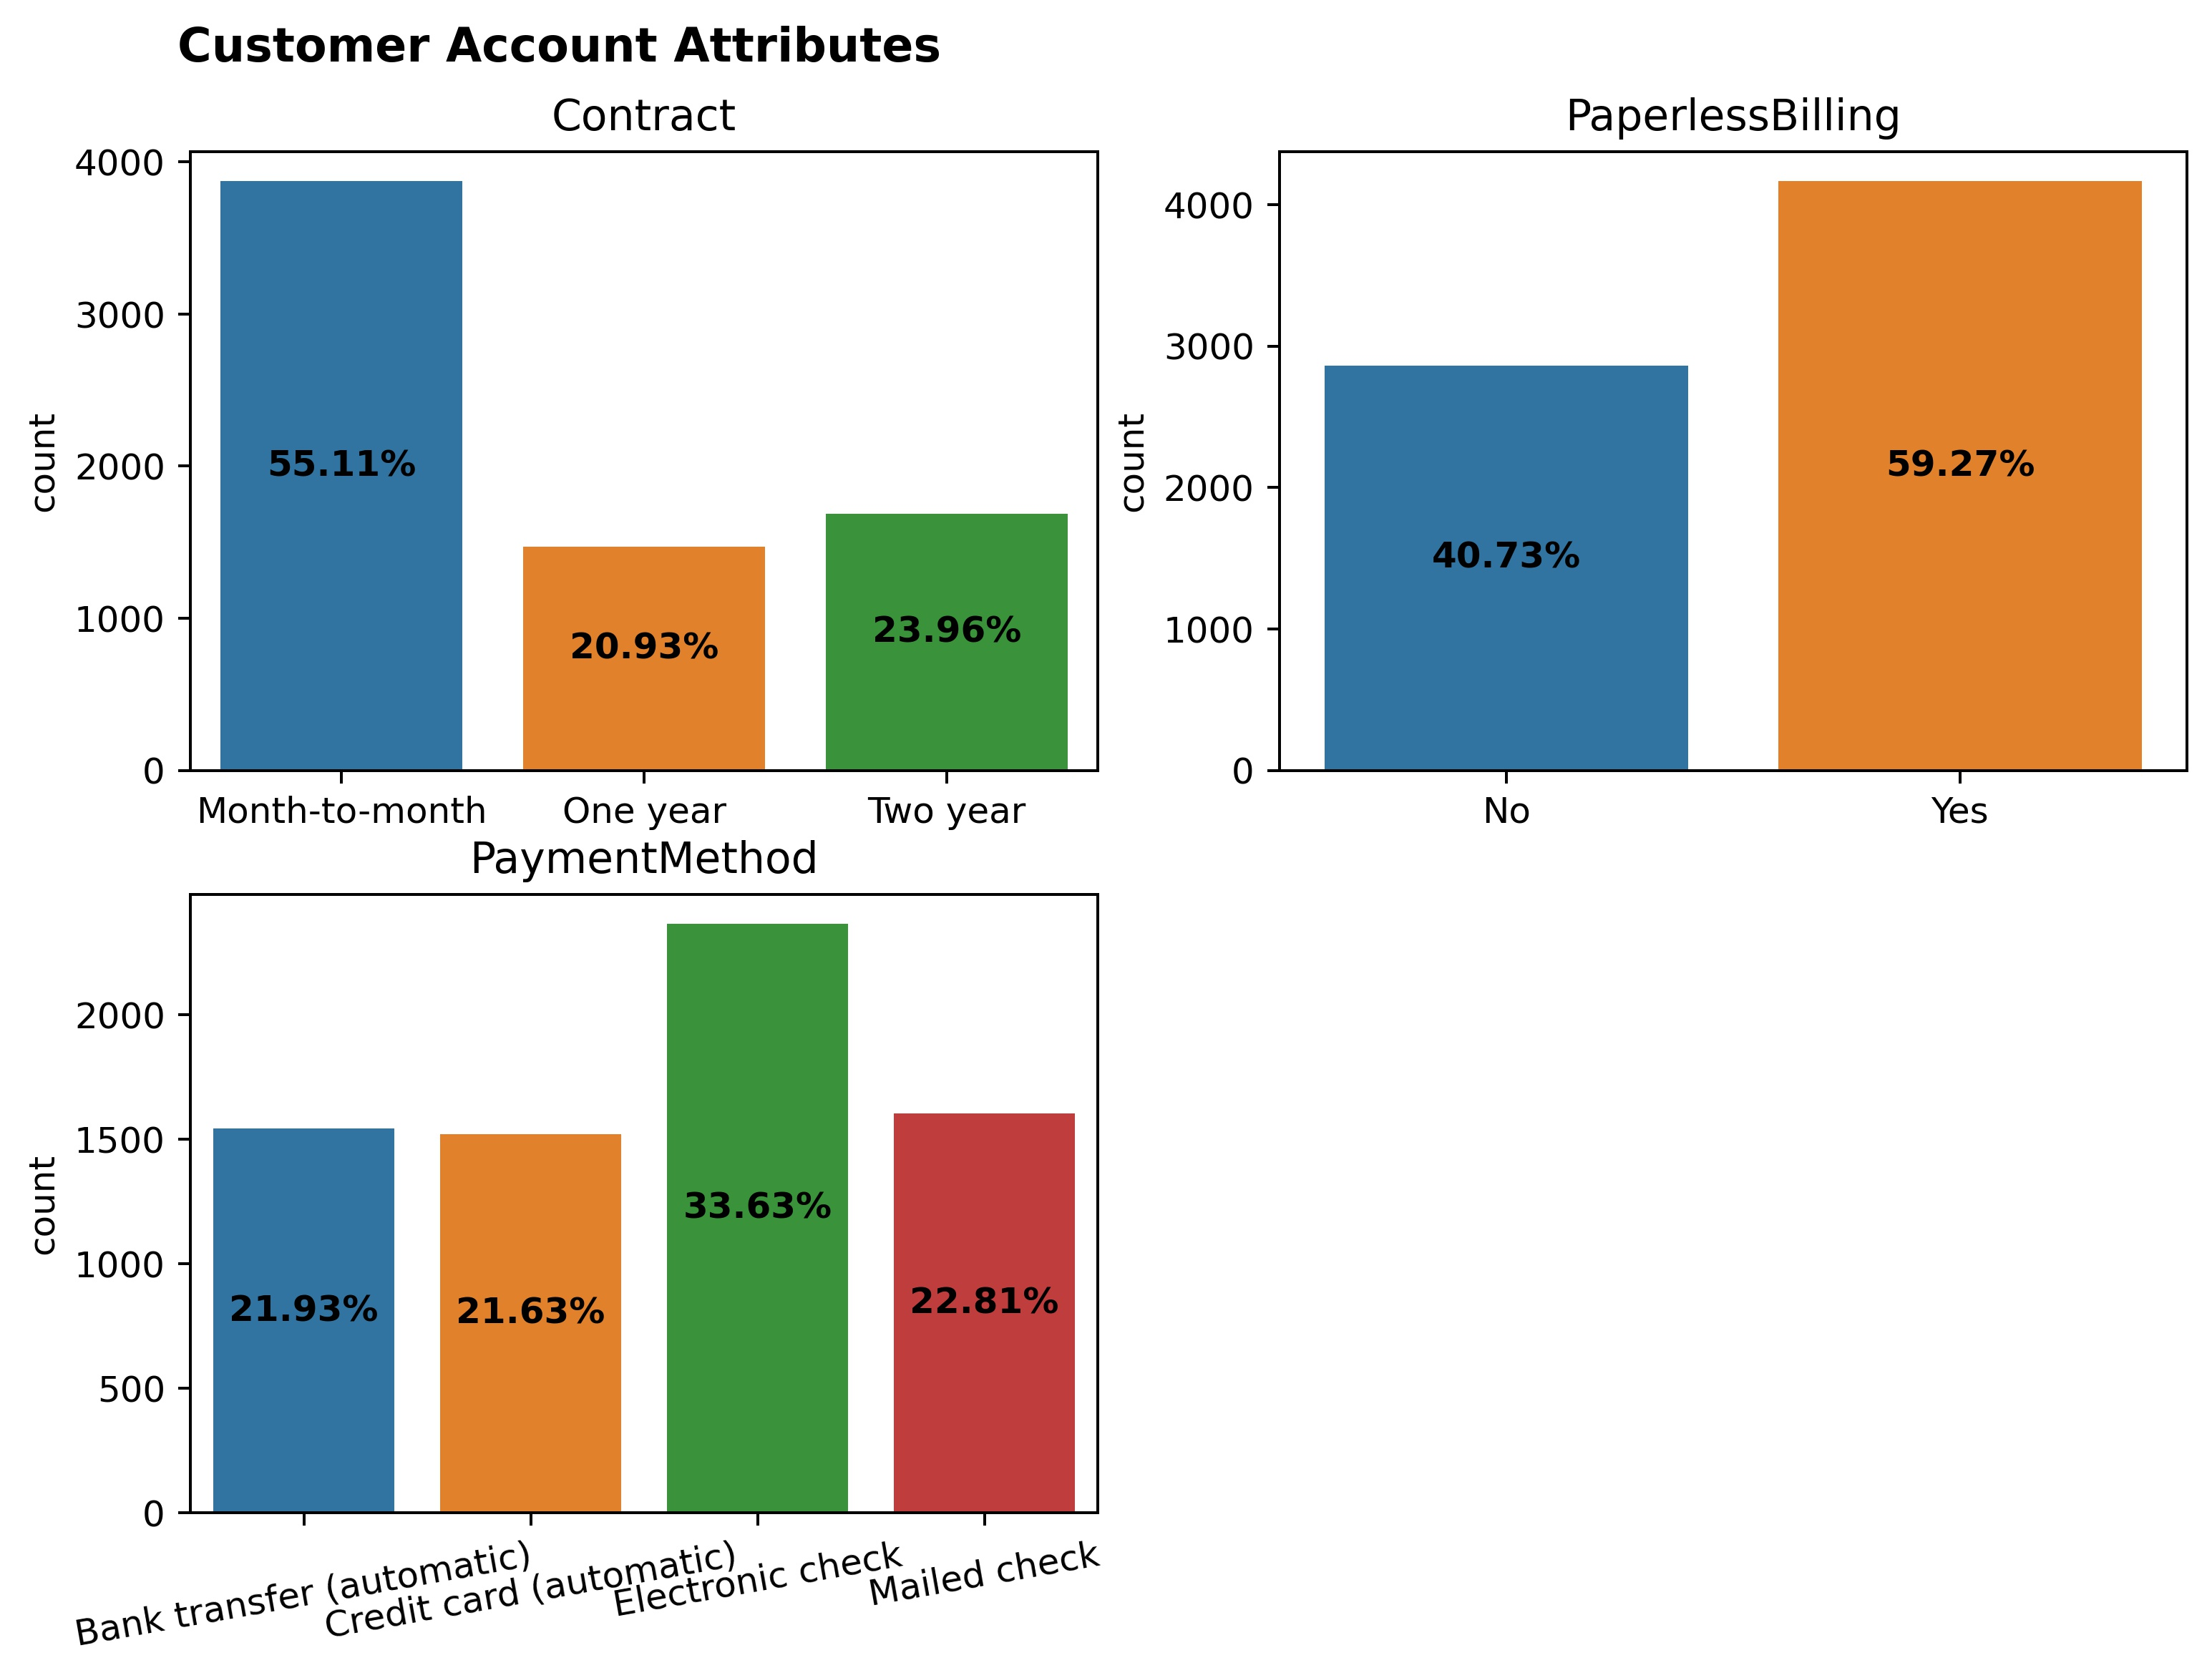
\includegraphics[width=1\linewidth]{figures/customer_acc}
	\caption{Univariate analysis of customer account attributes.}
	\label{fig:customer_acc}
\end{figure}

The last categorical variables such as Contract, PaperlessBilling, and Payment method give informations about customer account and transaction method. From Figure \ref{fig:customer_acc}, it is obvious that most customers prefer a month-to-month contract rather than a yearly contract. Moreover, for the transaction method, most customers opting for paperless billing and using electronic check.

\begin{figure}[t]
	\centering
	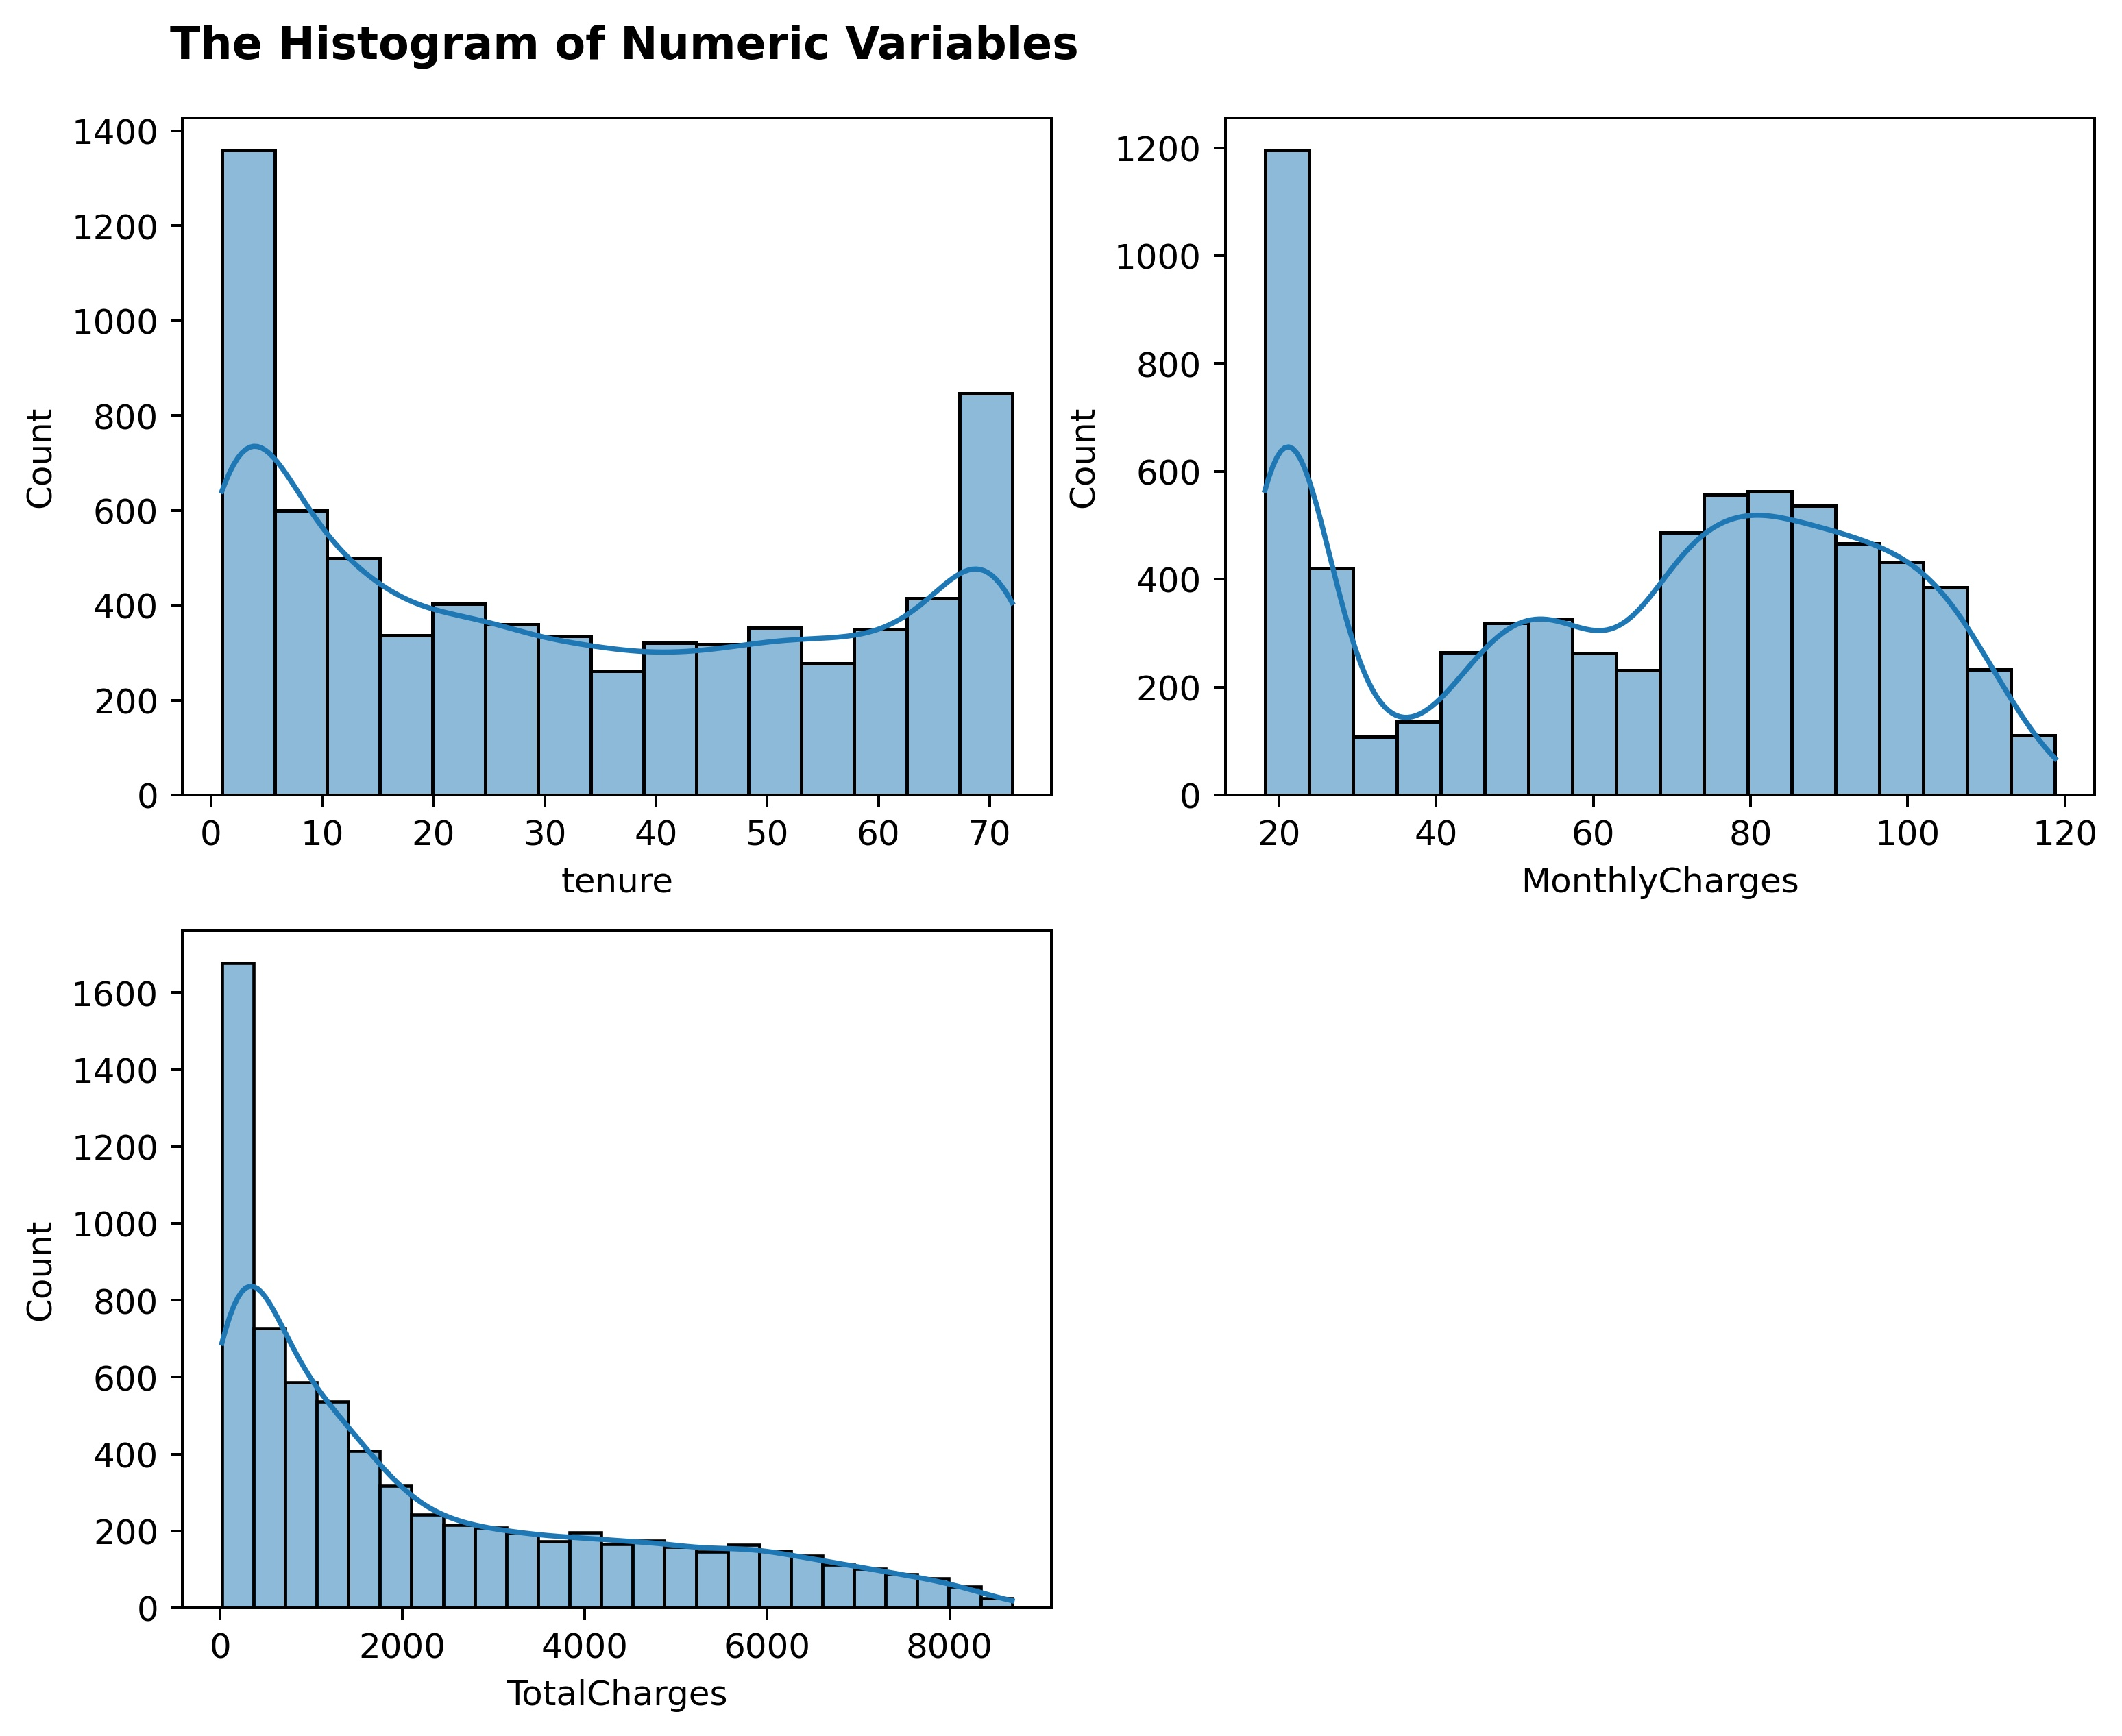
\includegraphics[width=1\linewidth]{figures/numeric_univ}
	\caption{Univariate analysis of numeric variables.}
	\label{fig:numeric_univ}
\end{figure}

For numeric variables, univariate analysis will be conducted using the histogram. In the preceding section, it is already known that there are no outliers in the dataset. However, the distribution of each variable is not yet known and needs to be visualized. From Figure \ref{fig:numeric_univ}, the tenure histogram shows that the distribution of its values is considered bi-modal (2 peaks), indicates that the dataset is concentrated around 2 clusters. One of them is customers with less than 10 months tenure and the last is loyal customers, signed up for 65 months or more. From another point of view, one can also see that the company has indeed been able to attract many customers in the last 10 months. The bimodal distribution is also visible in the MonthlyCharges distribution where the data set is focused around two groups, i.e customers who purchased the basic service (cheapest price) with the amount of 20 dollars only and other is the customer who purchased multi-services with the amount of approximately 80 dollars per month. Apart from its positively skewed form, it is difficult to interpret any useful information from the TotalCharges histogram since TotalCharges is roughly computed from MonthlyCharges multiplied by tenure. Since univariate analysis does not provide enough information to answer the problems, bivariate analysis will be conducted in the next section with great focus to the target variable, Churn.

\subsection{Bivariate Analysis}
In this section, the analysis will begin by calculating the correlation of each variable to another with the Spearman method. Before calculating the correlation matrix, the categorical variable within the dataset first need to be encoded. From Figure \ref{fig:spearmancor}, the result shows that tenure and MonthlyCharges are highly correlated to TotalCharges, which is reasonable since TotalCharges is roughly similar to MonthlyCharges multiplied by tenure. Other interesting result is encoded variable StreamingTV\_Yes has 0.53 correlation to StreamingMovies\_Yes, which indicates the customer who have TV streaming service is likely to have movies streaming service also. One also can see from the heatmap that services with strongest correlation to MonthlyCharges are fiber optic with 0.8, no internet service with -0.71 and streaming service with 0.64, describing those services do have strong influences to the MonthlyCharges value. Figure \ref{fig:spearmancor} also shows that Churn does not have quite strong correlation to any variable. The strongest correlations for the target variable Churn are -0.37 by tenure, 0.31 by fiber optic internet service, and 0.3 by electronic check.
\begin{landscape}
\begin{figure}[!htbp]
	\centering
	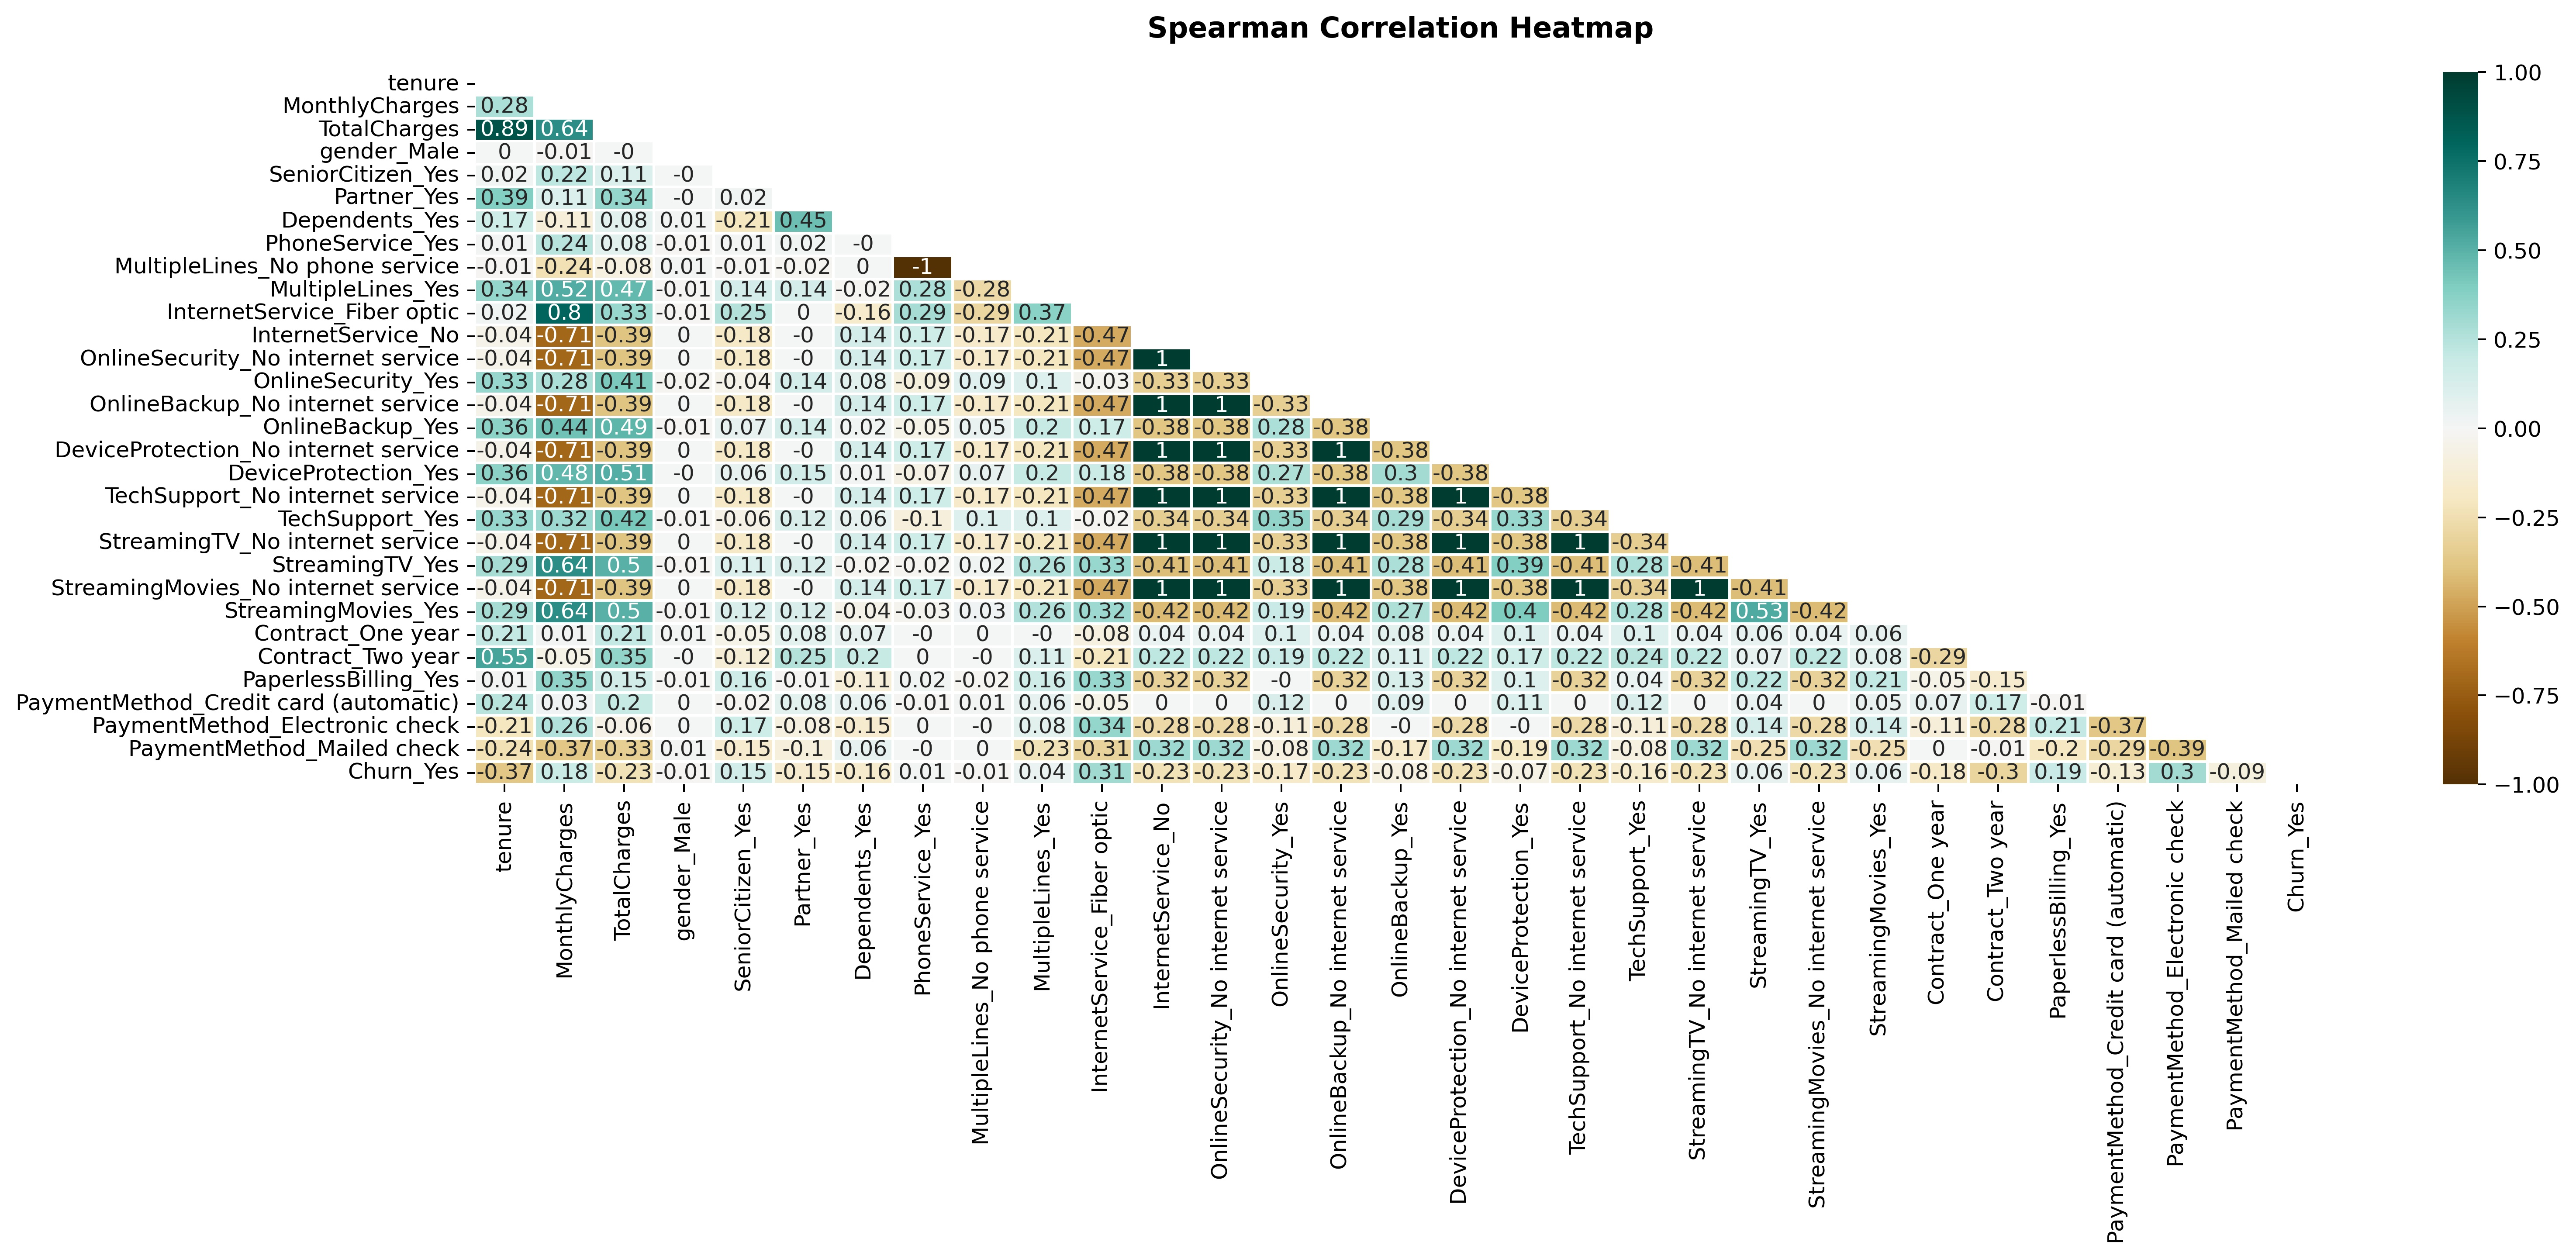
\includegraphics[width=25cm]{figures/spearman_cor}
	\caption{Spearman Correlation Heatmap for the encoded dataset.}
	\label{fig:spearmancor}
\end{figure}
\end{landscape}
 To obtain clearer picture of those correlations, the relationship between each variable and Churn will be visualized using stacked bar chart.
\begin{figure}[H]
	\centering
	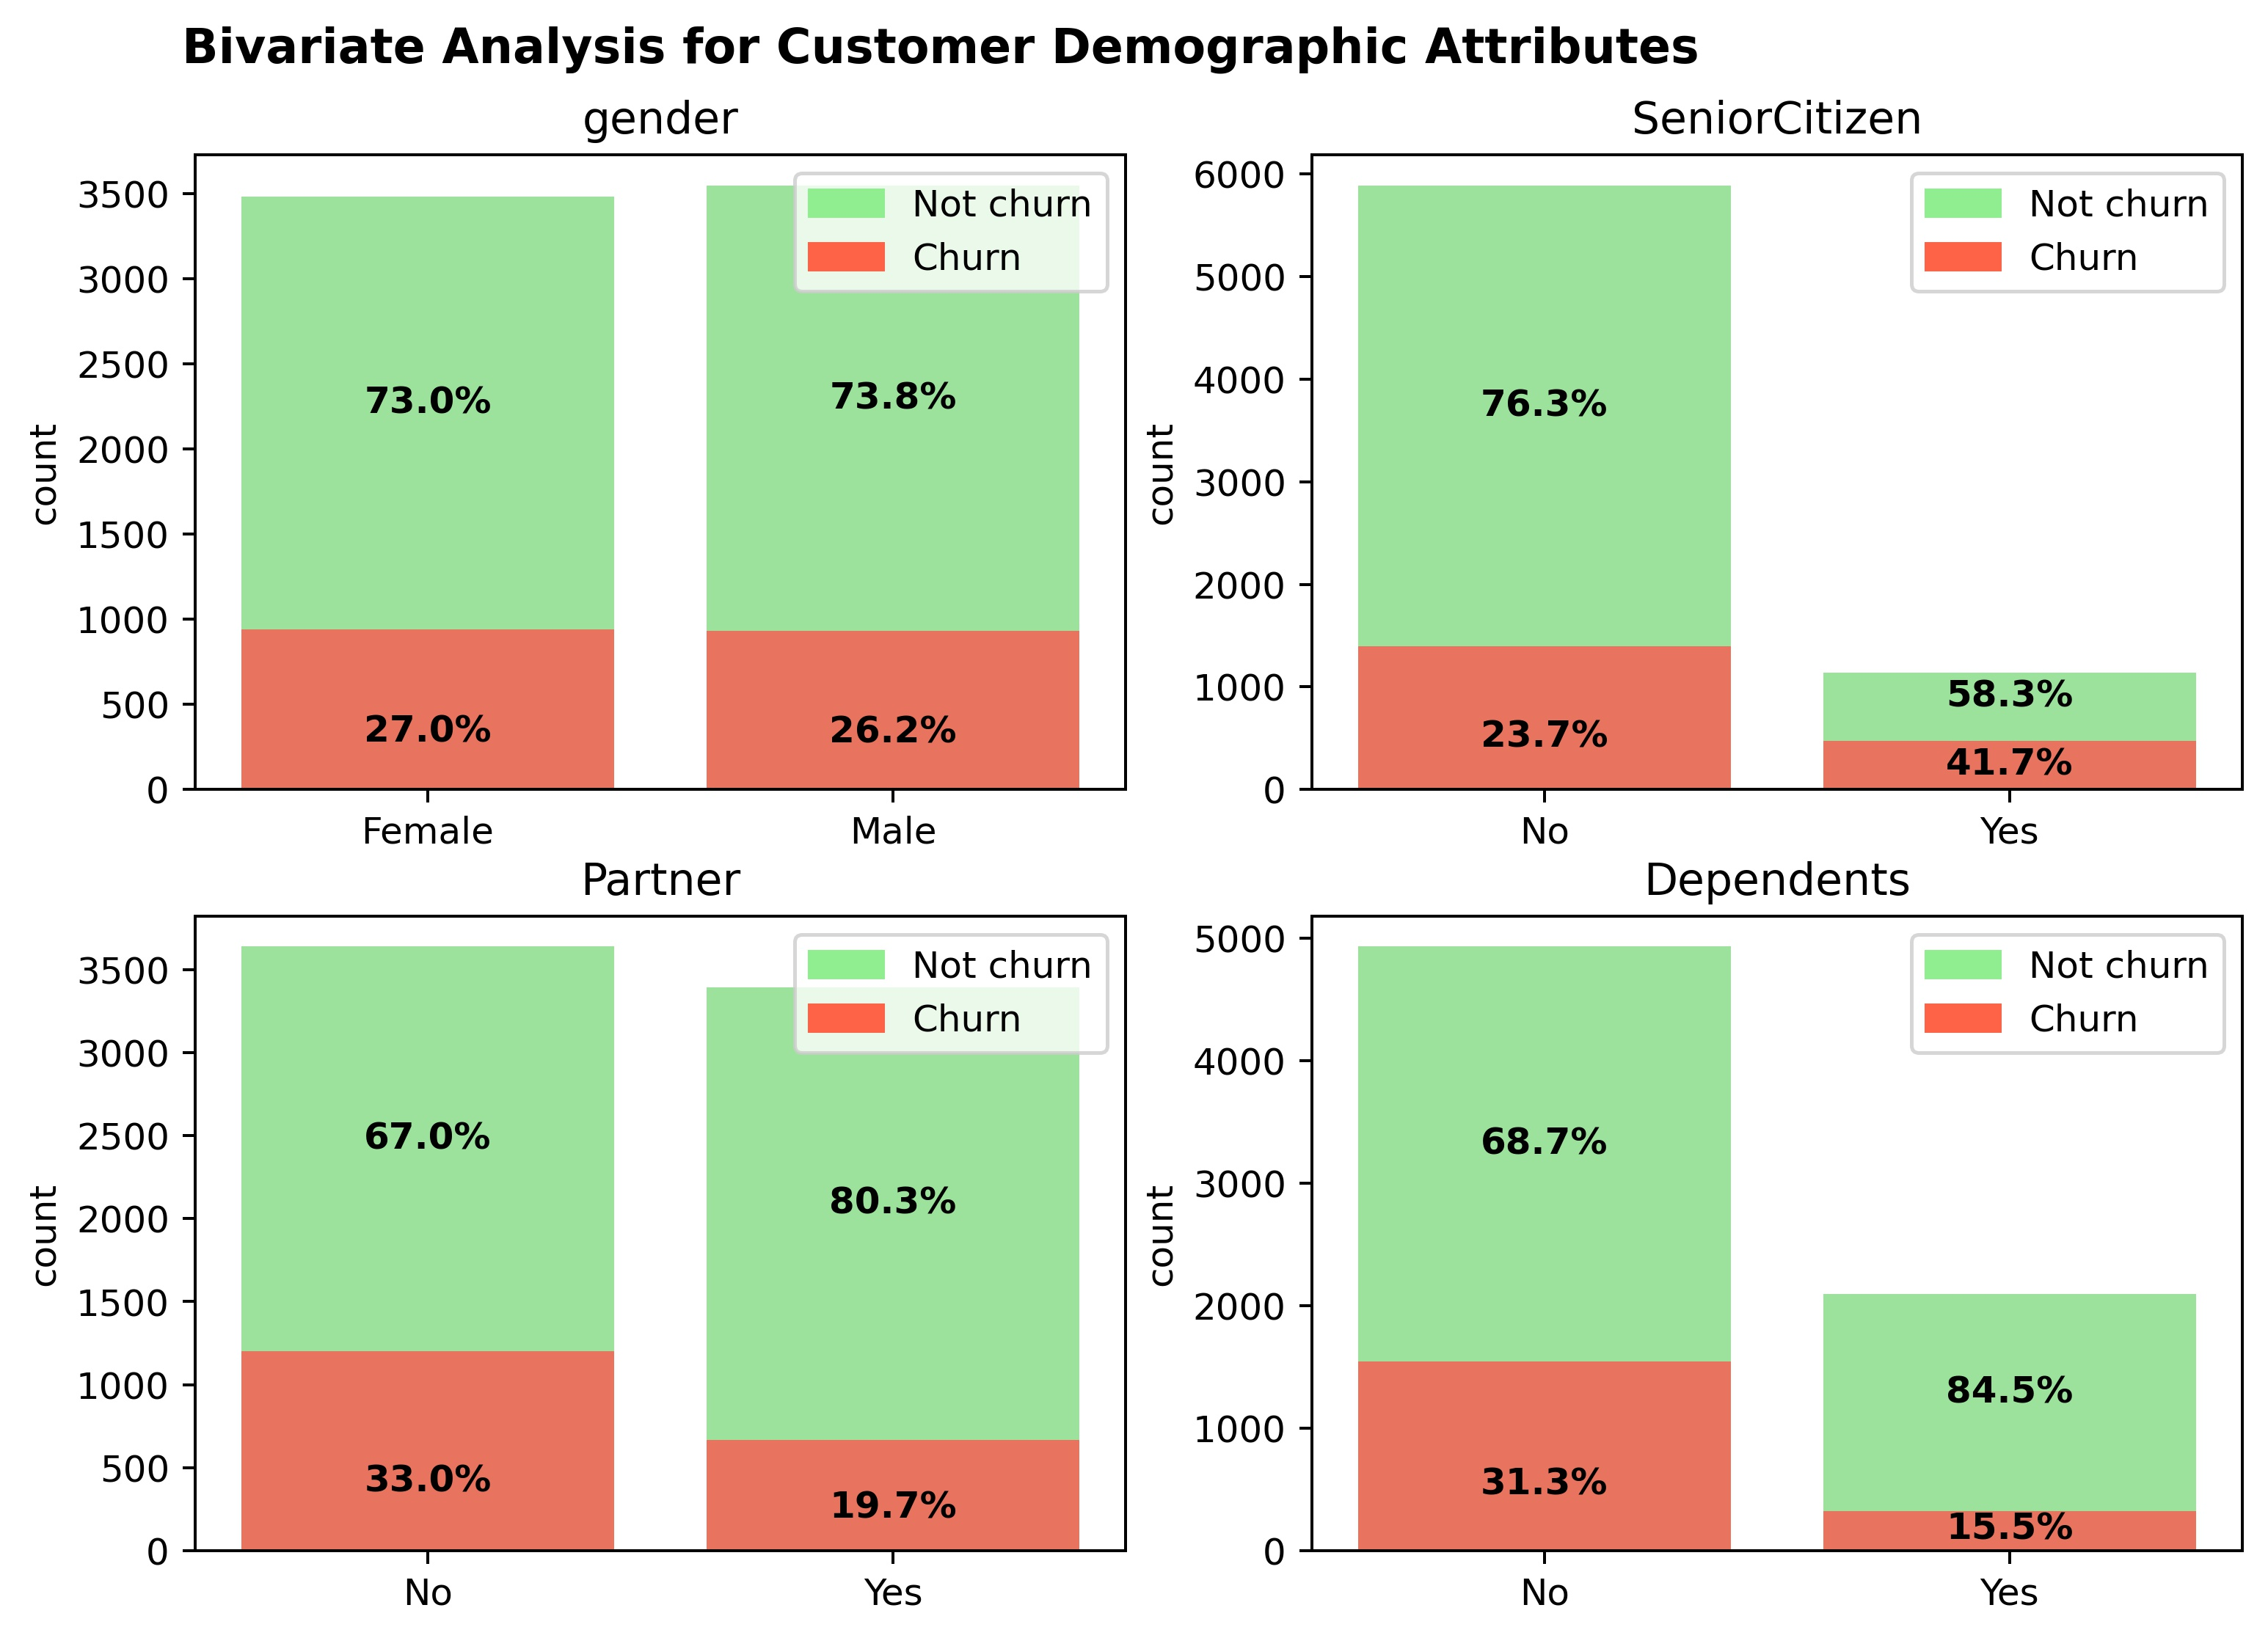
\includegraphics[width=0.8\linewidth]{figures/customer_demo_bi}
	\caption{Bivariate Analysis of Customer Demographic Attributes and Churn.}
	\label{fig:customer_demo_bi}
\end{figure}

\begin{figure}[H]
	\centering
	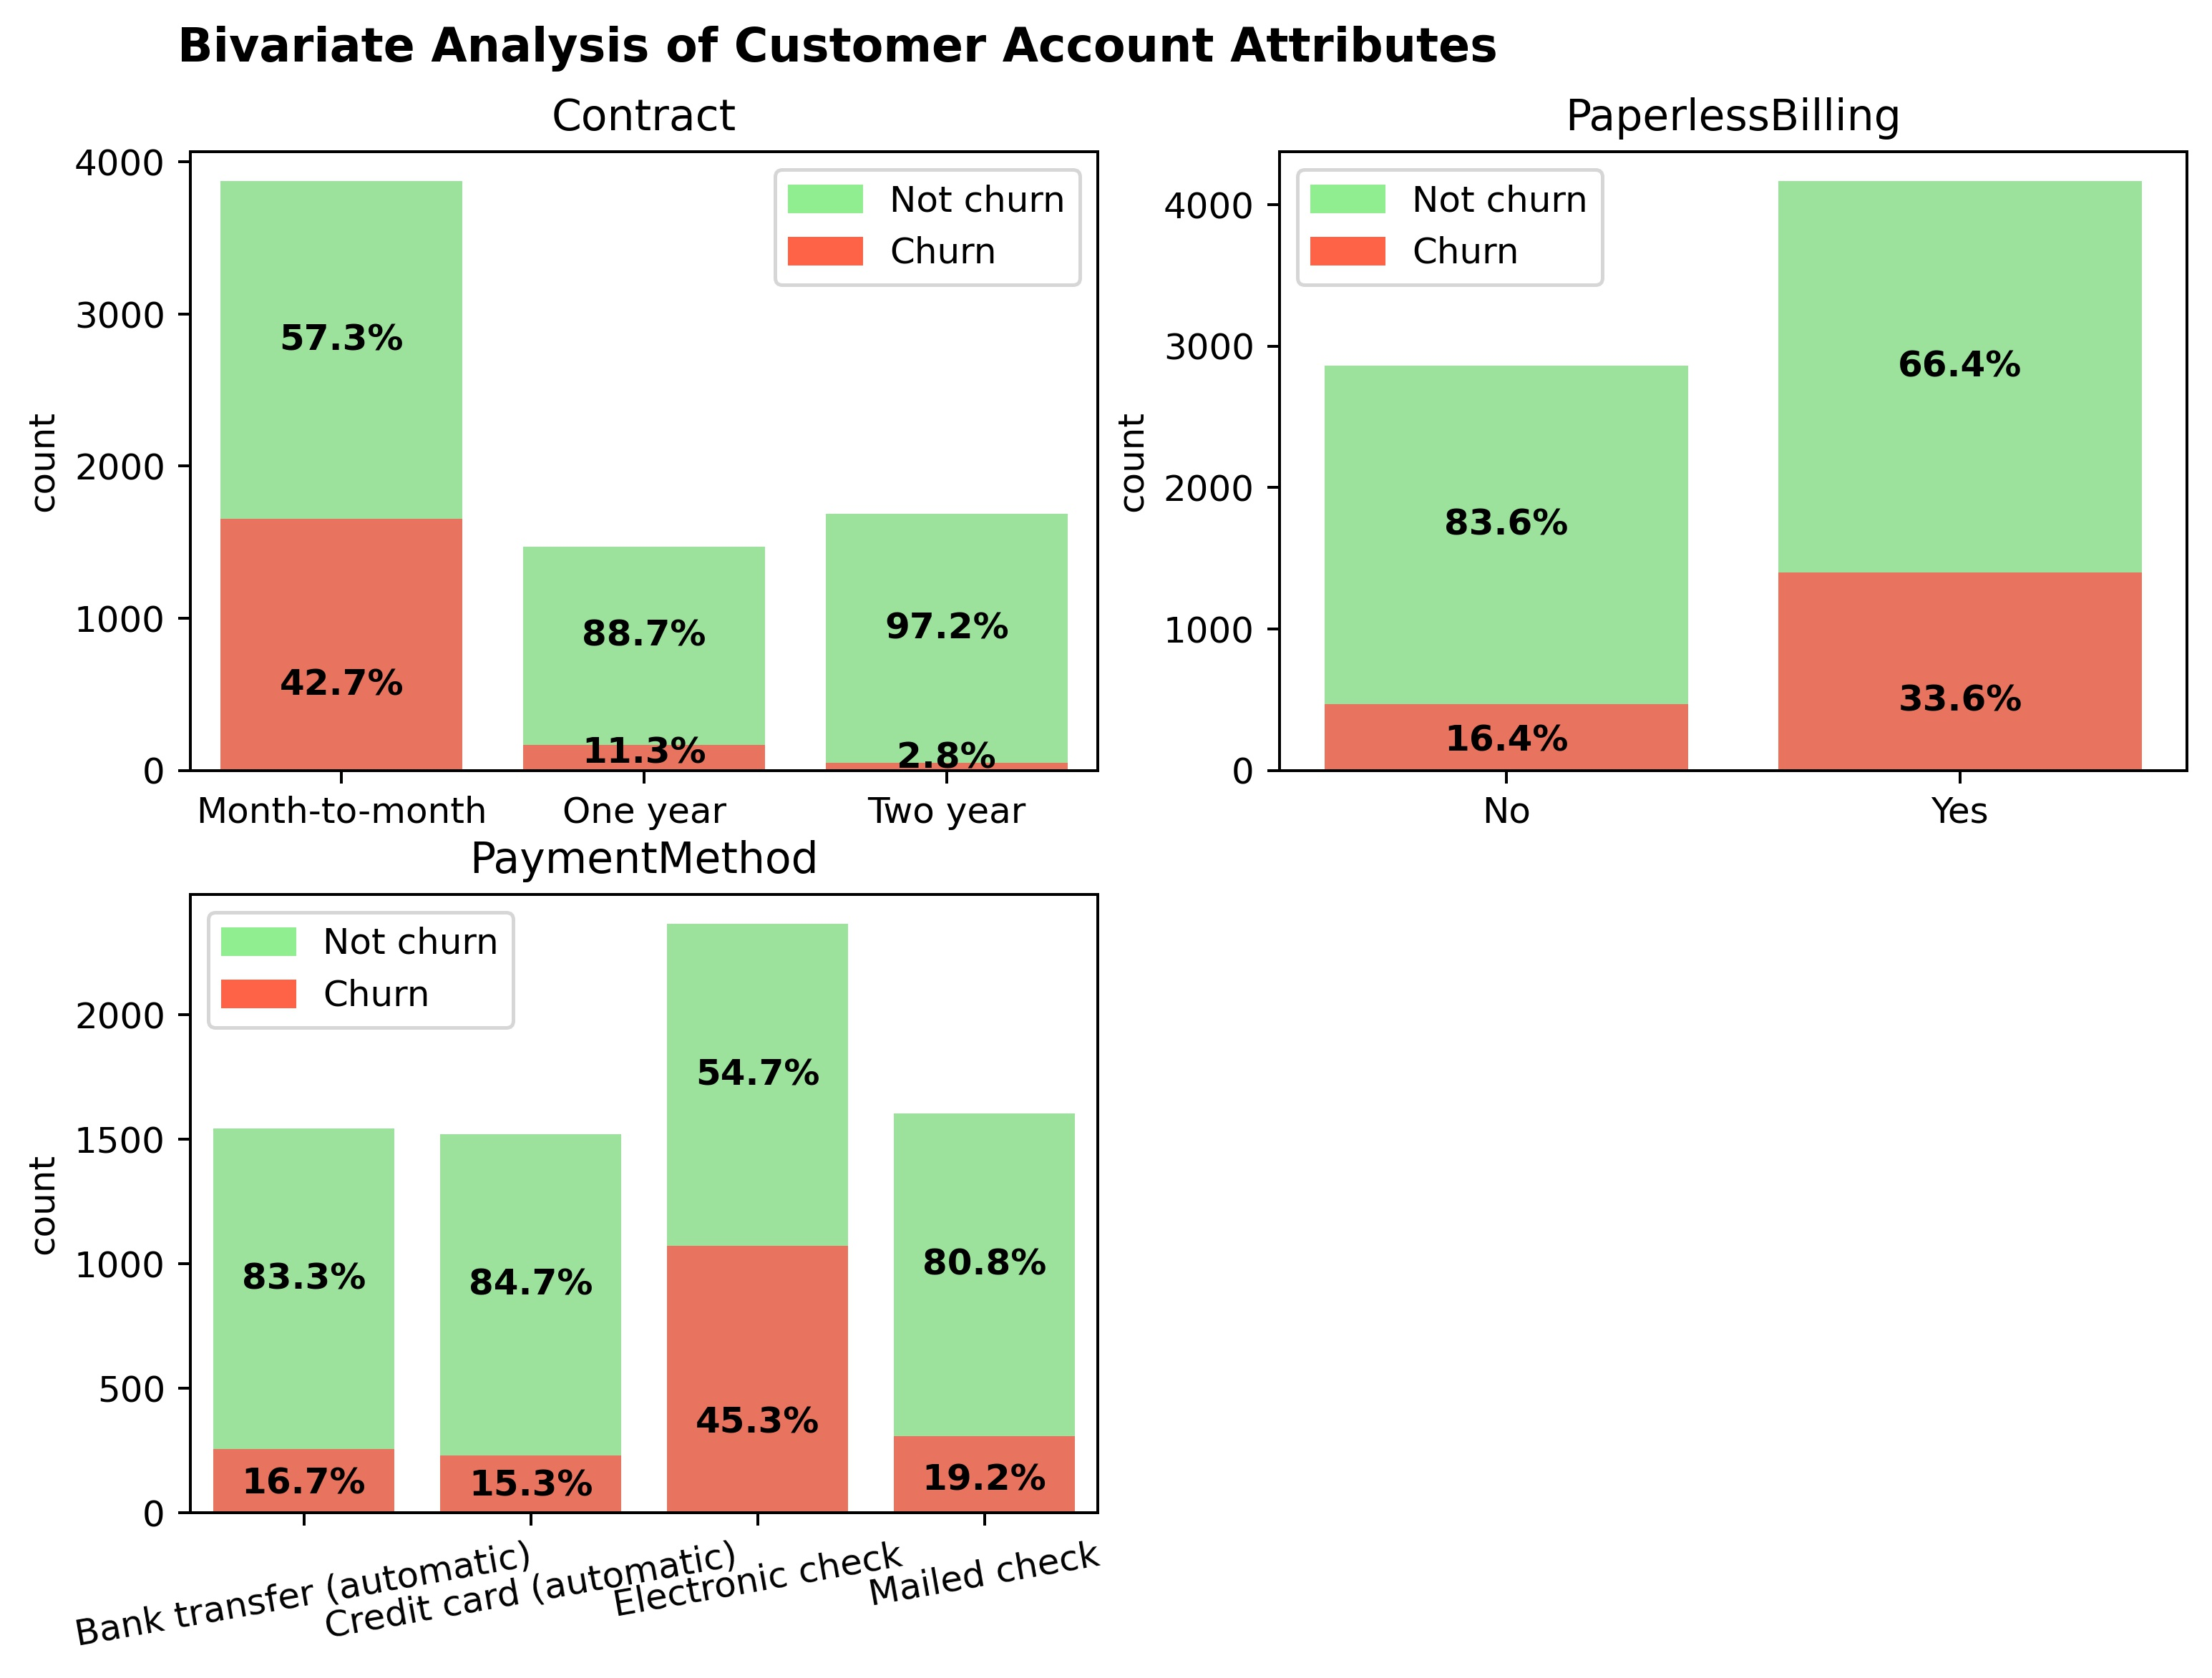
\includegraphics[width=0.8\linewidth]{figures/customer_acc_bi}
	\caption{Bivariate Analysis of Customer Account Attributes and Churn.}
	\label{fig:customer_acc_bi}
\end{figure}

\begin{figure}[H]
	\centering
	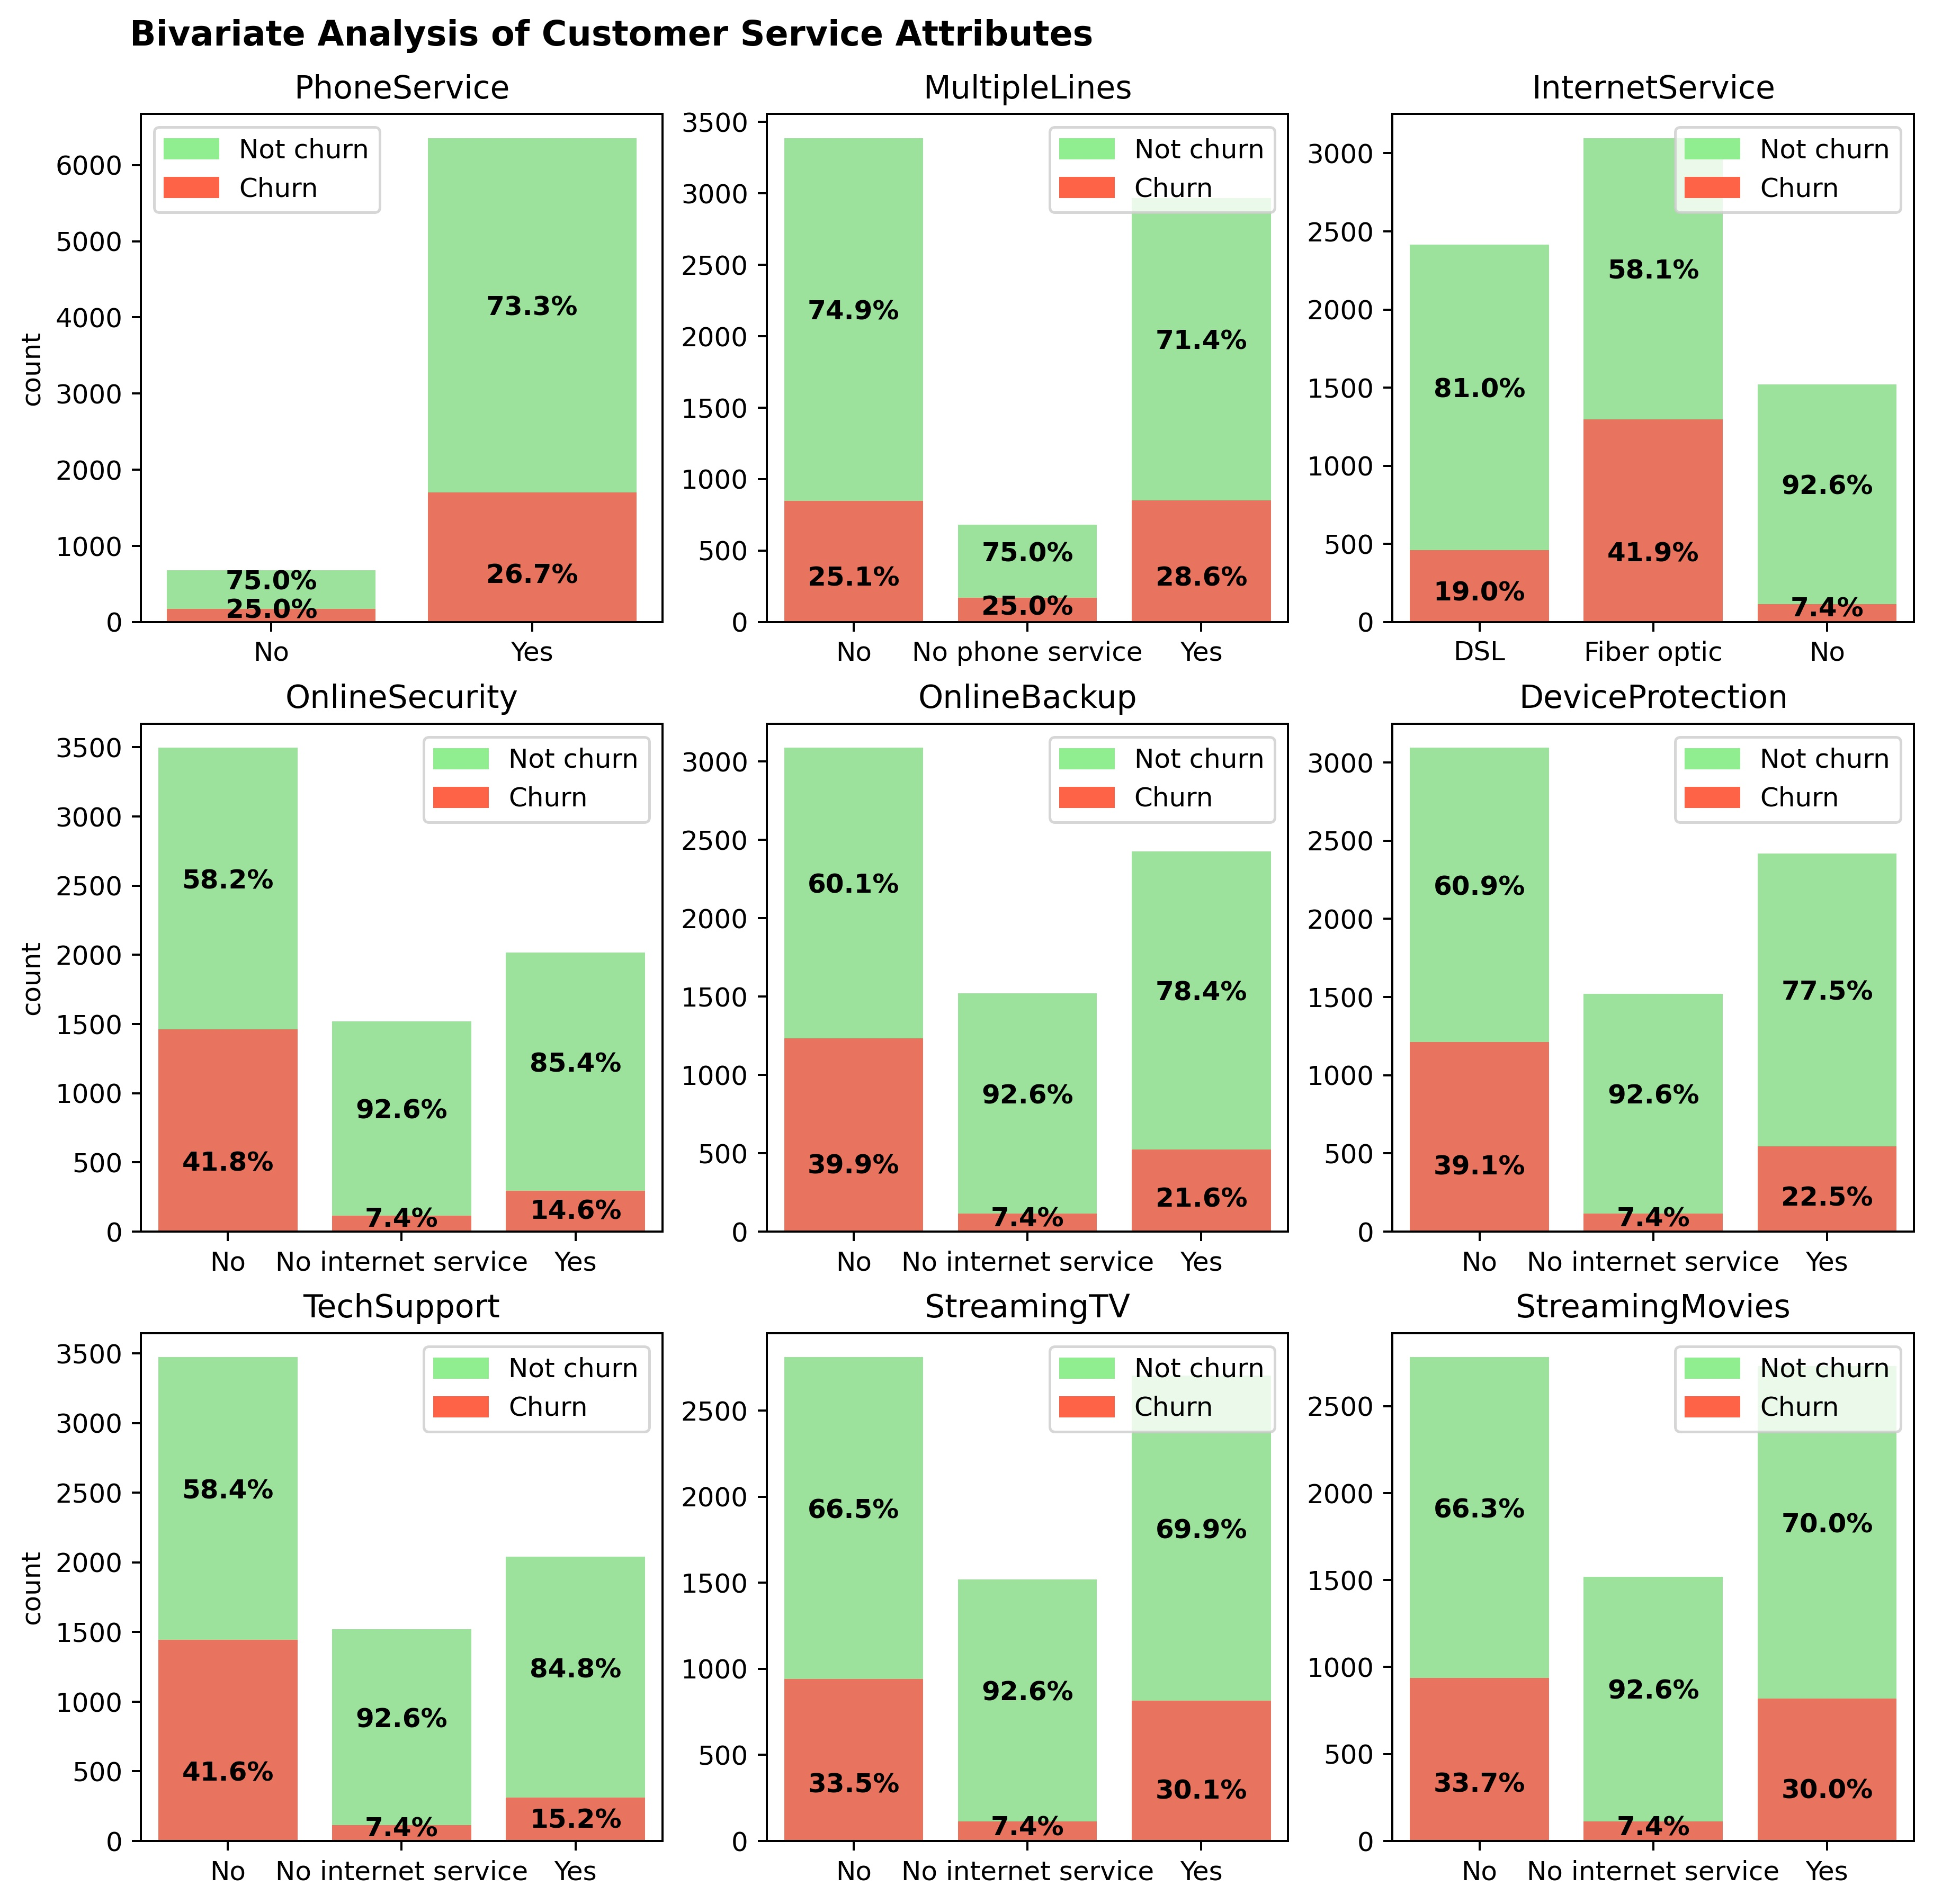
\includegraphics[width=1\linewidth]{figures/customer_service_bi}
	\caption{Bivariate Analysis of Customer Service Attributes and Churn.}
	\label{fig:customer_service_bi}
\end{figure}
 From the stacked bar charts of customer demographic attributes, customer account attributes, and customer service attributes (Figure \ref{fig:customer_demo_bi}, \ref{fig:customer_acc_bi}, \ref{fig:customer_service_bi}) one can notice that :
\begin{itemize}
	\item Both sexes, female and male have the same likelihood to churn, meaning that this variable don't give any valuable pieces of information. Same thing does not apply for Partner and Dependents since bar charts show that customer who has partner or dependents is less likely to churn. Bar chart also shows that senior customer has bigger chance to churn than younger one.
	\item Figure \ref{fig:customer_acc_bi} shows that customer with monthly subscription has greater chance to churn than customer with yearly subscription. The bar charts also show customers with paperless billing enabled and has electronic check for payment method are more likely to churn.
	\item From customer service attributes, it can be seen that roughly 40\% of customers who sign up for the fiber optic service choose to churn, meanwhile more than 90\% of customers who don't sign up for the internet service choose to remain. Moreover, it seems that customer who does not subscribe for additional internet services such as OnlineSecurity, OnlineBackup, DeviceProtection, and TechSupport has greater chance to churn than customer who subscribes. Same thing does not apply for both streaming services, since the churn probability of customer with or without streaming services enabled is roughly equal by 30\%. This value is considered high compared to OnlineSecurity, OnlineBackup and so on, indicating that numerous customers might less satisfied with the quality of the streaming services.
\end{itemize}

\begin{figure}[!hb]
	\centering
	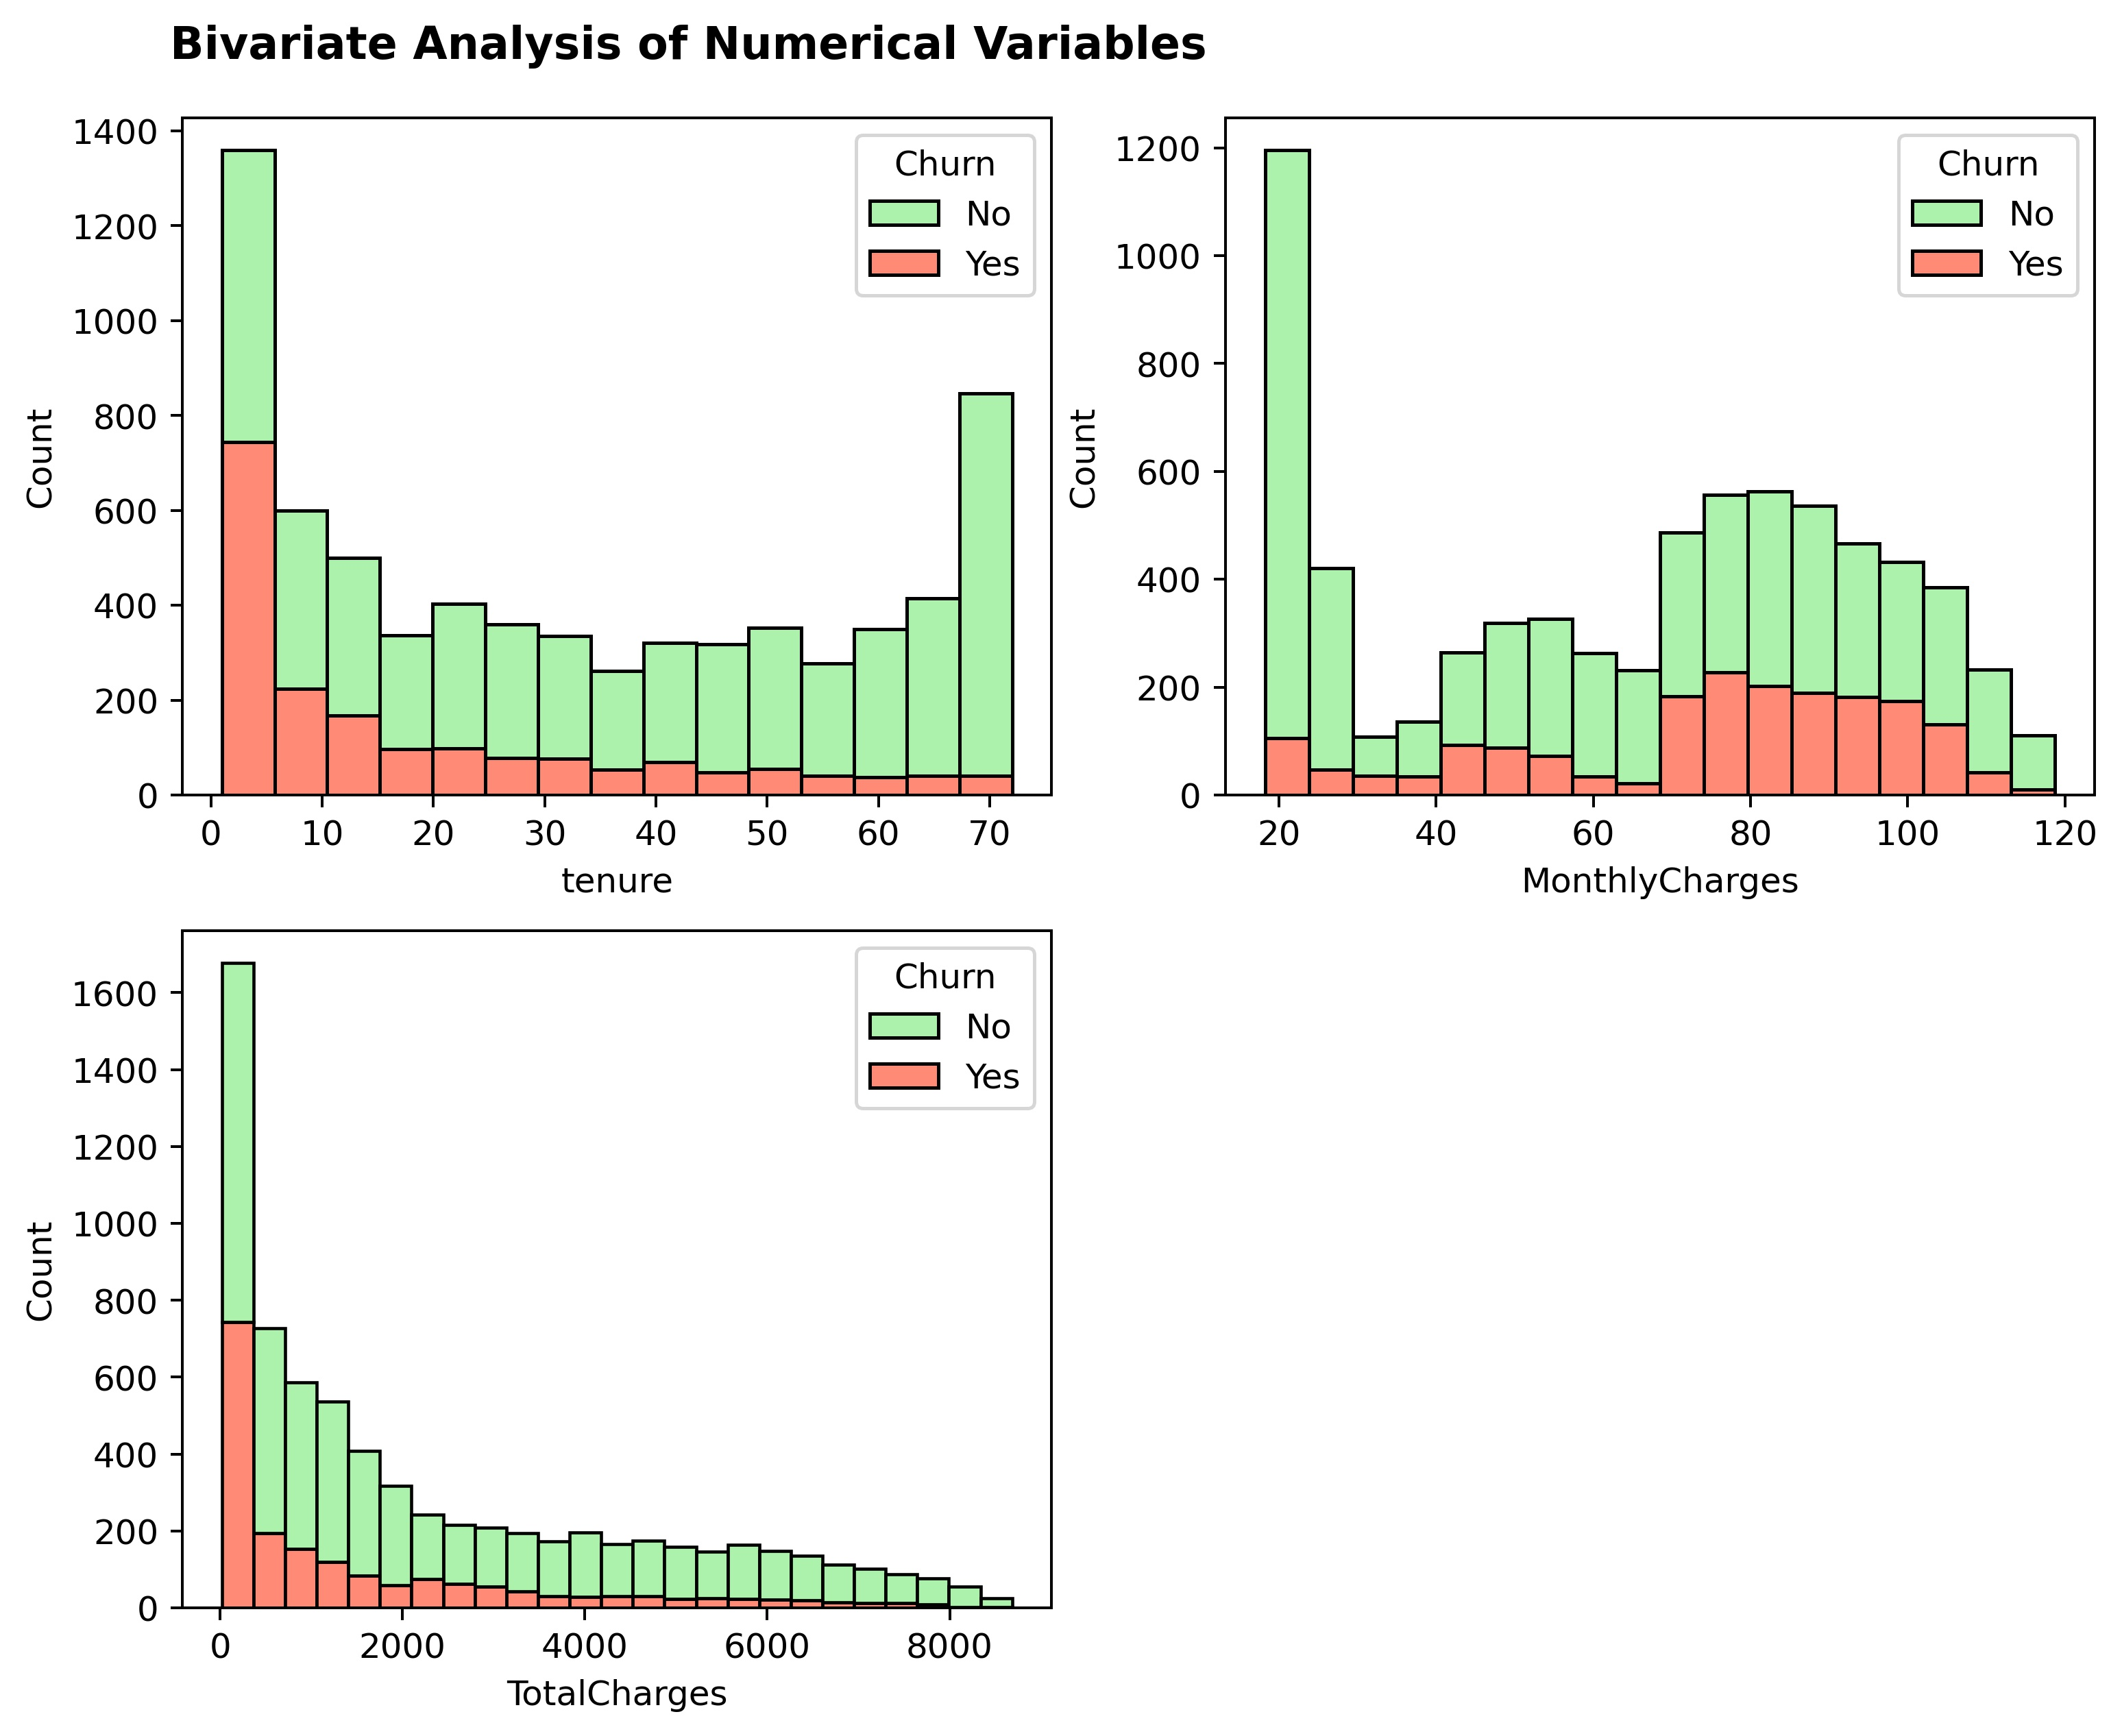
\includegraphics[width=1\linewidth]{figures/num_var_bi}
	\caption{Bivariate Analysis of Numerical Variables.}
	\label{fig:num_var_bi}
\end{figure}
The bivariate analysis will also be conducted for the numerical variables such as tenure, MonthlyCharges, and TotalCharges. Figure \ref{fig:num_var_bi} shows that most customers who churned within the last month only subscribed for less than 5 months. This is definitely a loss as the company has actually managed to attract a lot of new customers in the last few months. From MonthlyCharges histogram, it appears that the majority of lost customers are charged by approximately 70-110 dollars per month. To urge more detail information, these 2 variables will be binned by dividing their values into 6 quantiles with roughly similar amount. 
\begin{figure}[!htbp]
	\centering
	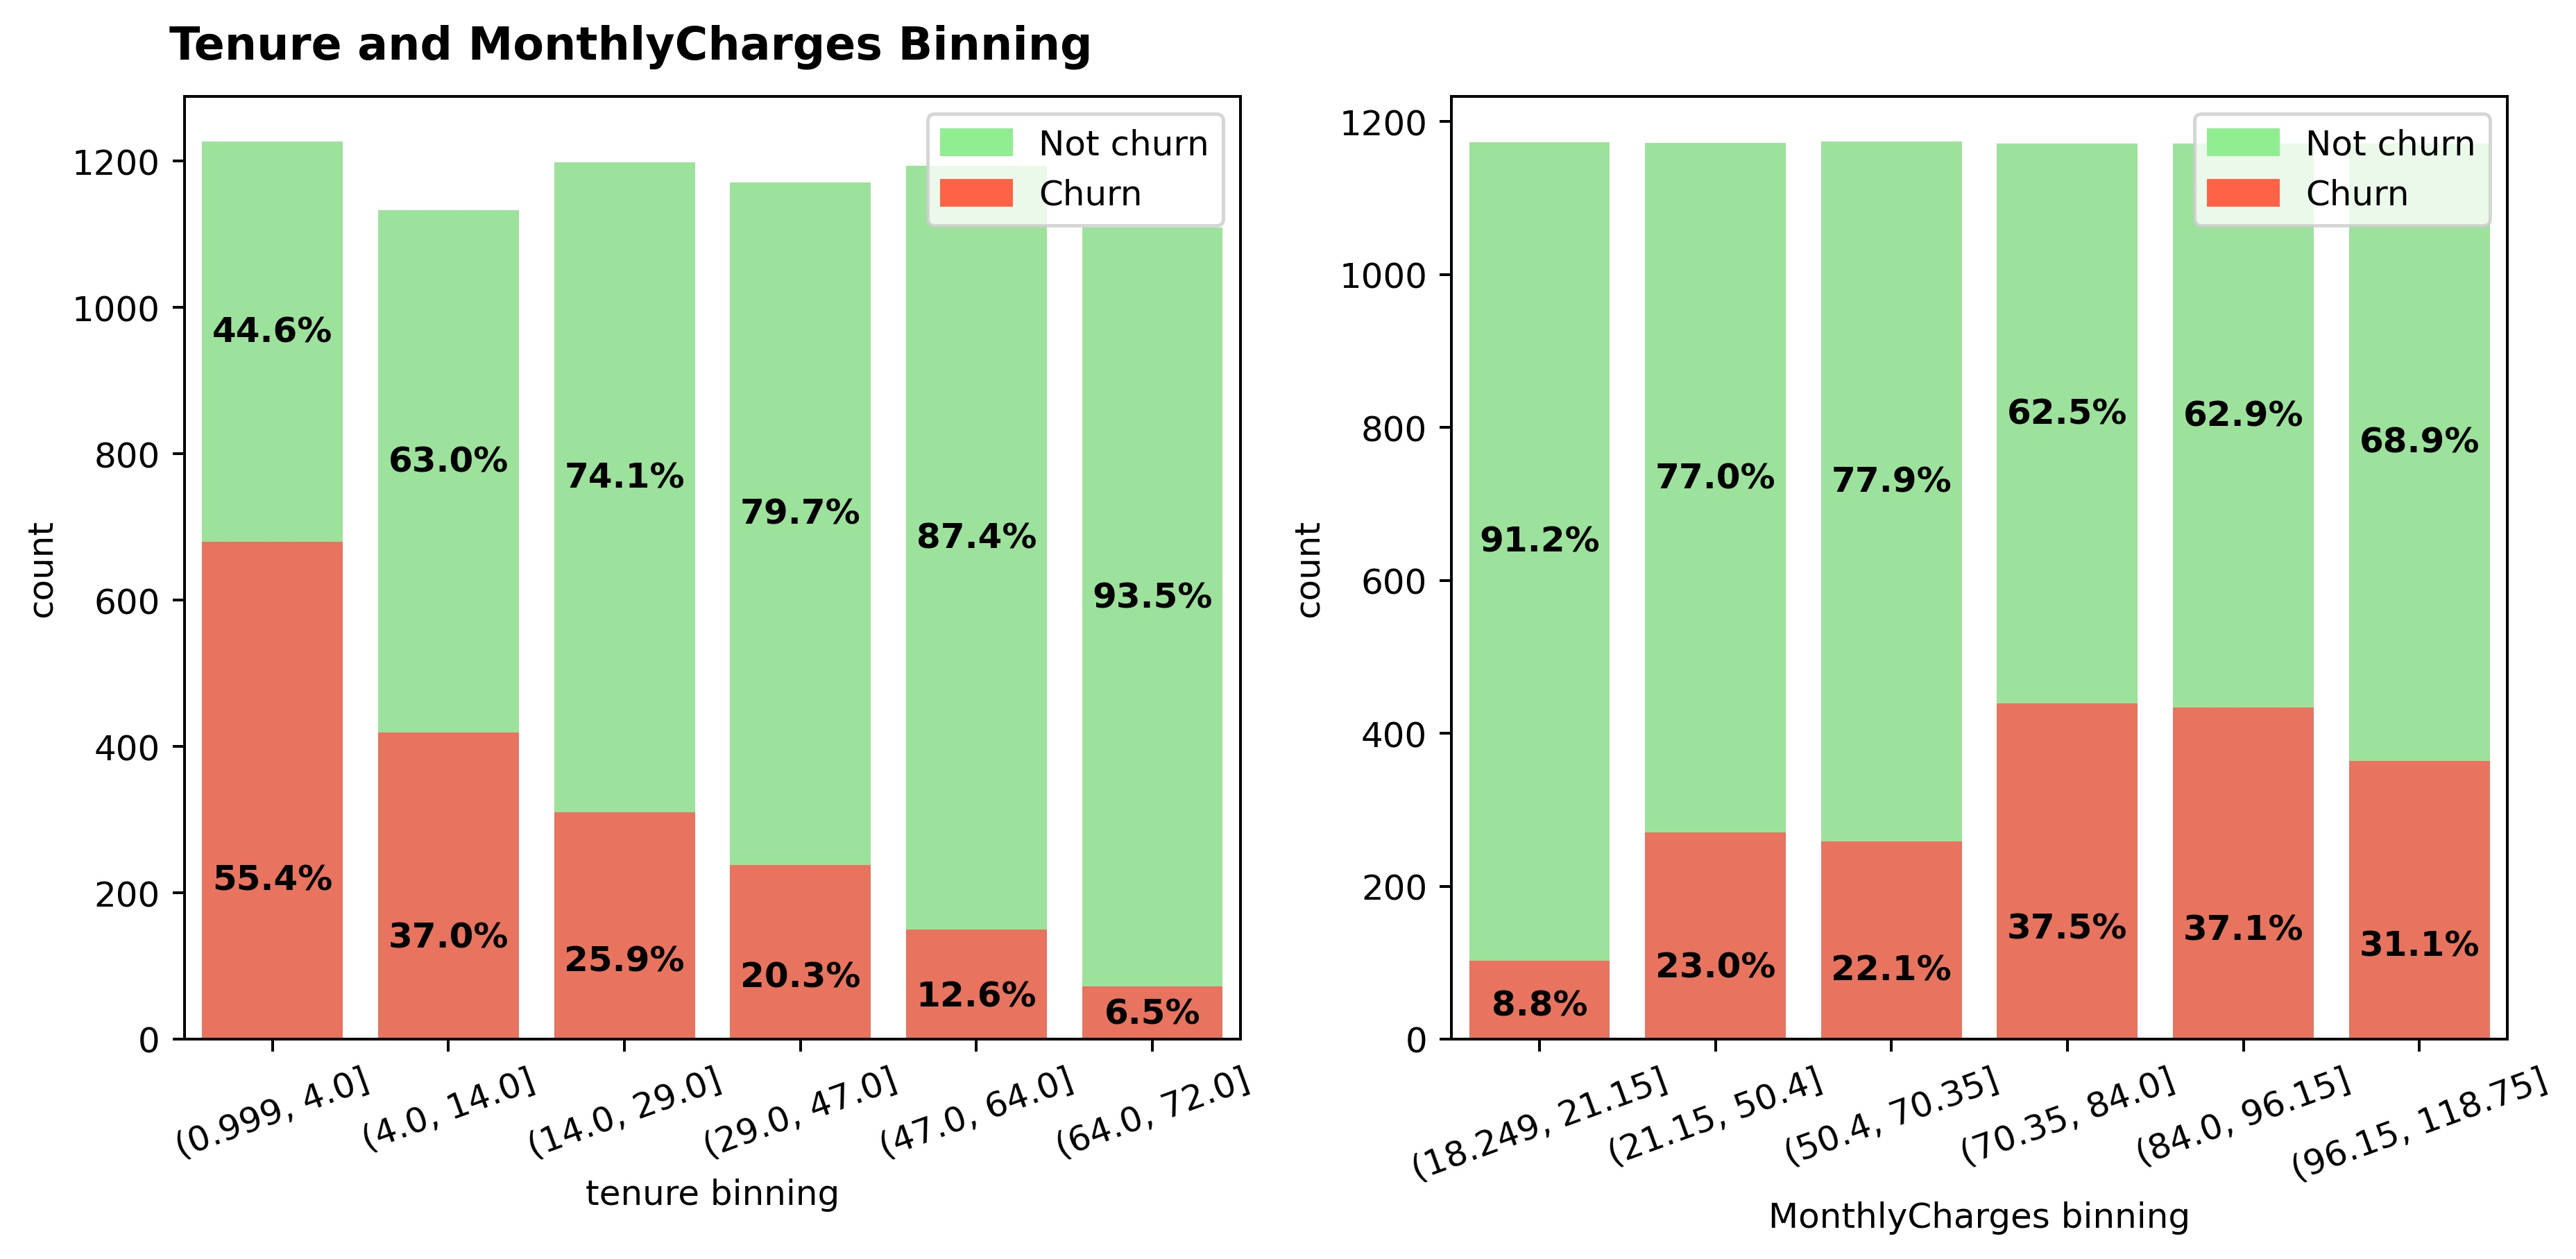
\includegraphics[width=1\linewidth]{figures/binning}
	\caption{Discretization of MonthlyCharges and tenure.}
	\label{fig:binning}
\end{figure}
Figure \ref{fig:binning} appears an instinctive result as the churn likelihood gets smaller as the membership time gets longer. It also tells that more than 50\% of customers who only subscribed less than 4 months prefer to churn (mostly even churn in their first month). From MonthlyCharges binning, it can be seen that the premium customers who are billed more than 70 dollars per month are more likely to churn compared to other customers with less bill. From the business perspective, it is surely more beneficial for the company to have a great focus improving on the premium services since those services have more lost customers and donate more month-to-month income for the company. Another interesting result is the customer who only subscribes for basic service seems quite satistied with the service quality and less likely to churn.

\subsection{Summary and Justification}
From bivariate analysis, one can figure several categories that may represent who the lost customer is. However, the question of which factors is the main culprit remains unanswered. Consider that it is impossible for customers who use electronic check for the payment method decide to churn without any reasons. In this section, that question will be tried to solve.
\begin{figure}[!htbp]
	\centering
	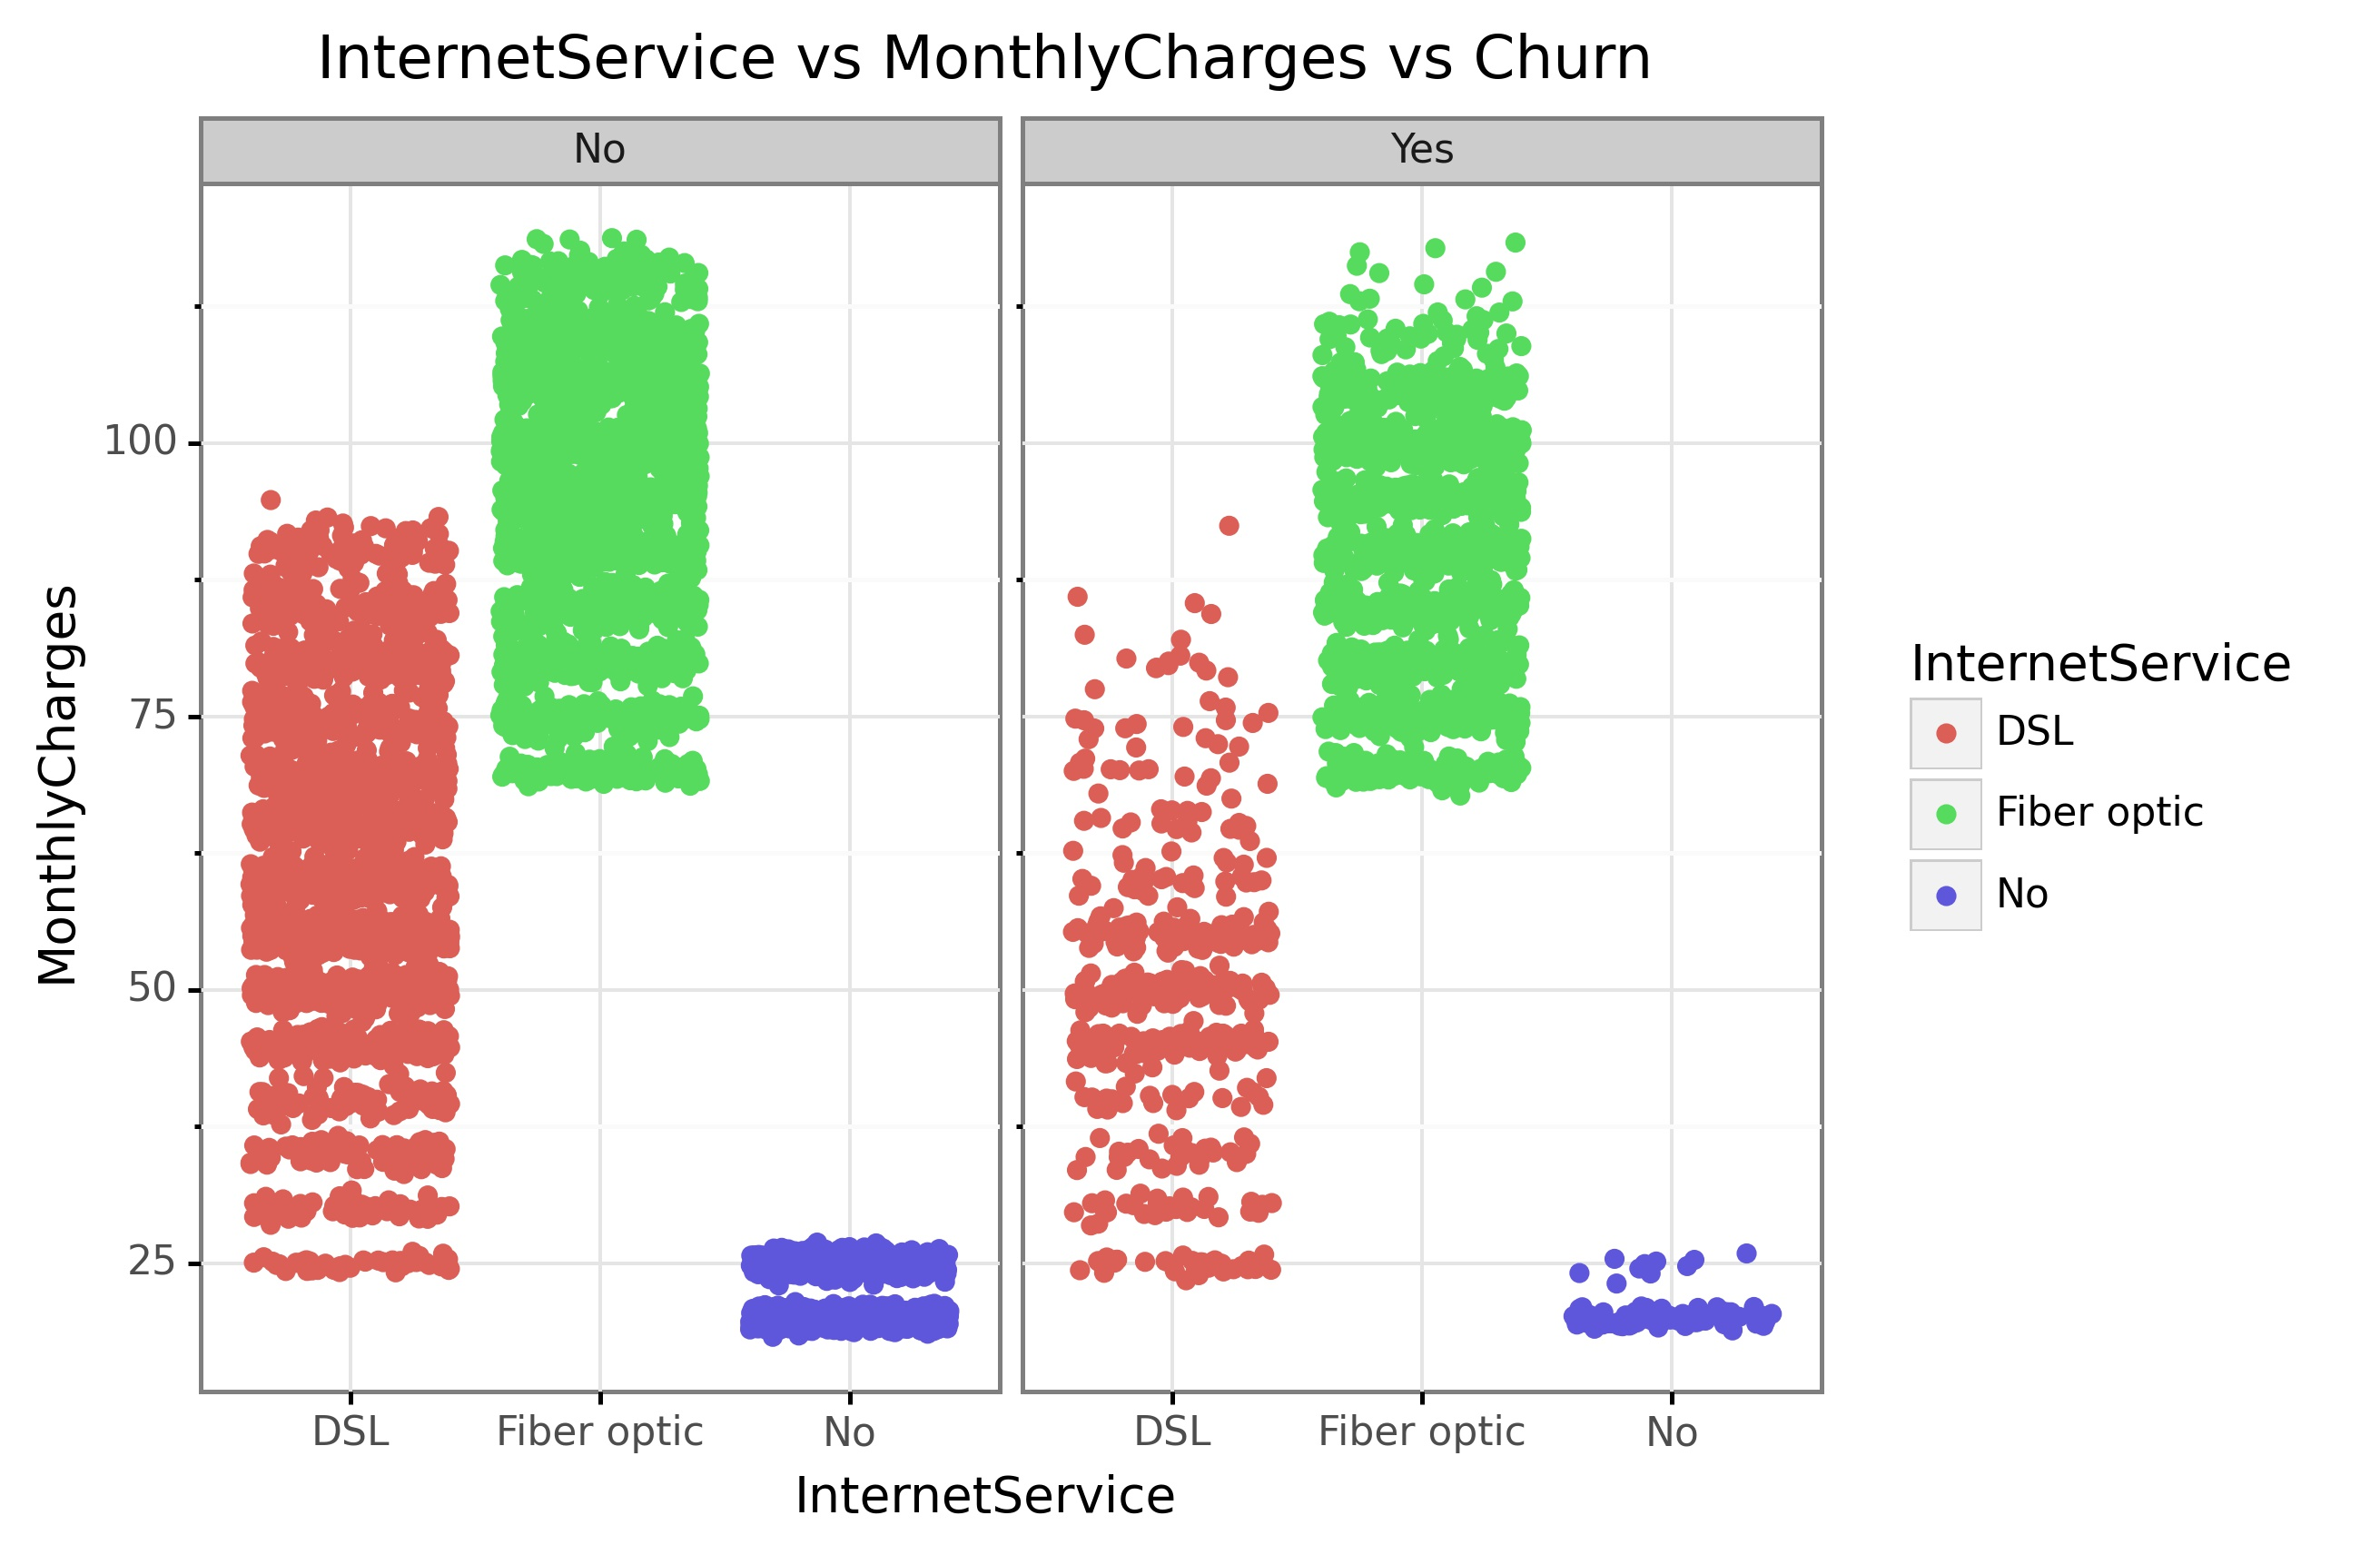
\includegraphics[width=0.7\linewidth]{figures/justifi_monthly}
	\caption{Jitter plot of InternetService vs MonthlyCharges vs Churn.}
	\label{fig:justify_monthly}
\end{figure}

Figure \ref{fig:justify_monthly} depicts why many customers who pay more than 70 dollars per month choose to churn. The reason is due to the internet service they bought.  As shown in Figure \ref{fig:justify_monthly}, it is evident that customers who churn with MonthlyCharges ranging from 70 to 120 dollars are usually customers who use FiberOptic service. From the previous section, one of the most important insights is Fiber Optic service indeed has higher rate of churn. That's also why SeniorCitizen, ElectronicCheck, and PaperlessBilling have higher churn rates than others. Figure \ref{fig:justify_sc} shows that MonthlyCharges distribution for SeniorCitizen Yes, PaperlessBilling Yes and Electronic check are clustered around the churn-critical area, i.e 60-90 dollars per month. 

\begin{figure}[!htbp]
	\centering
	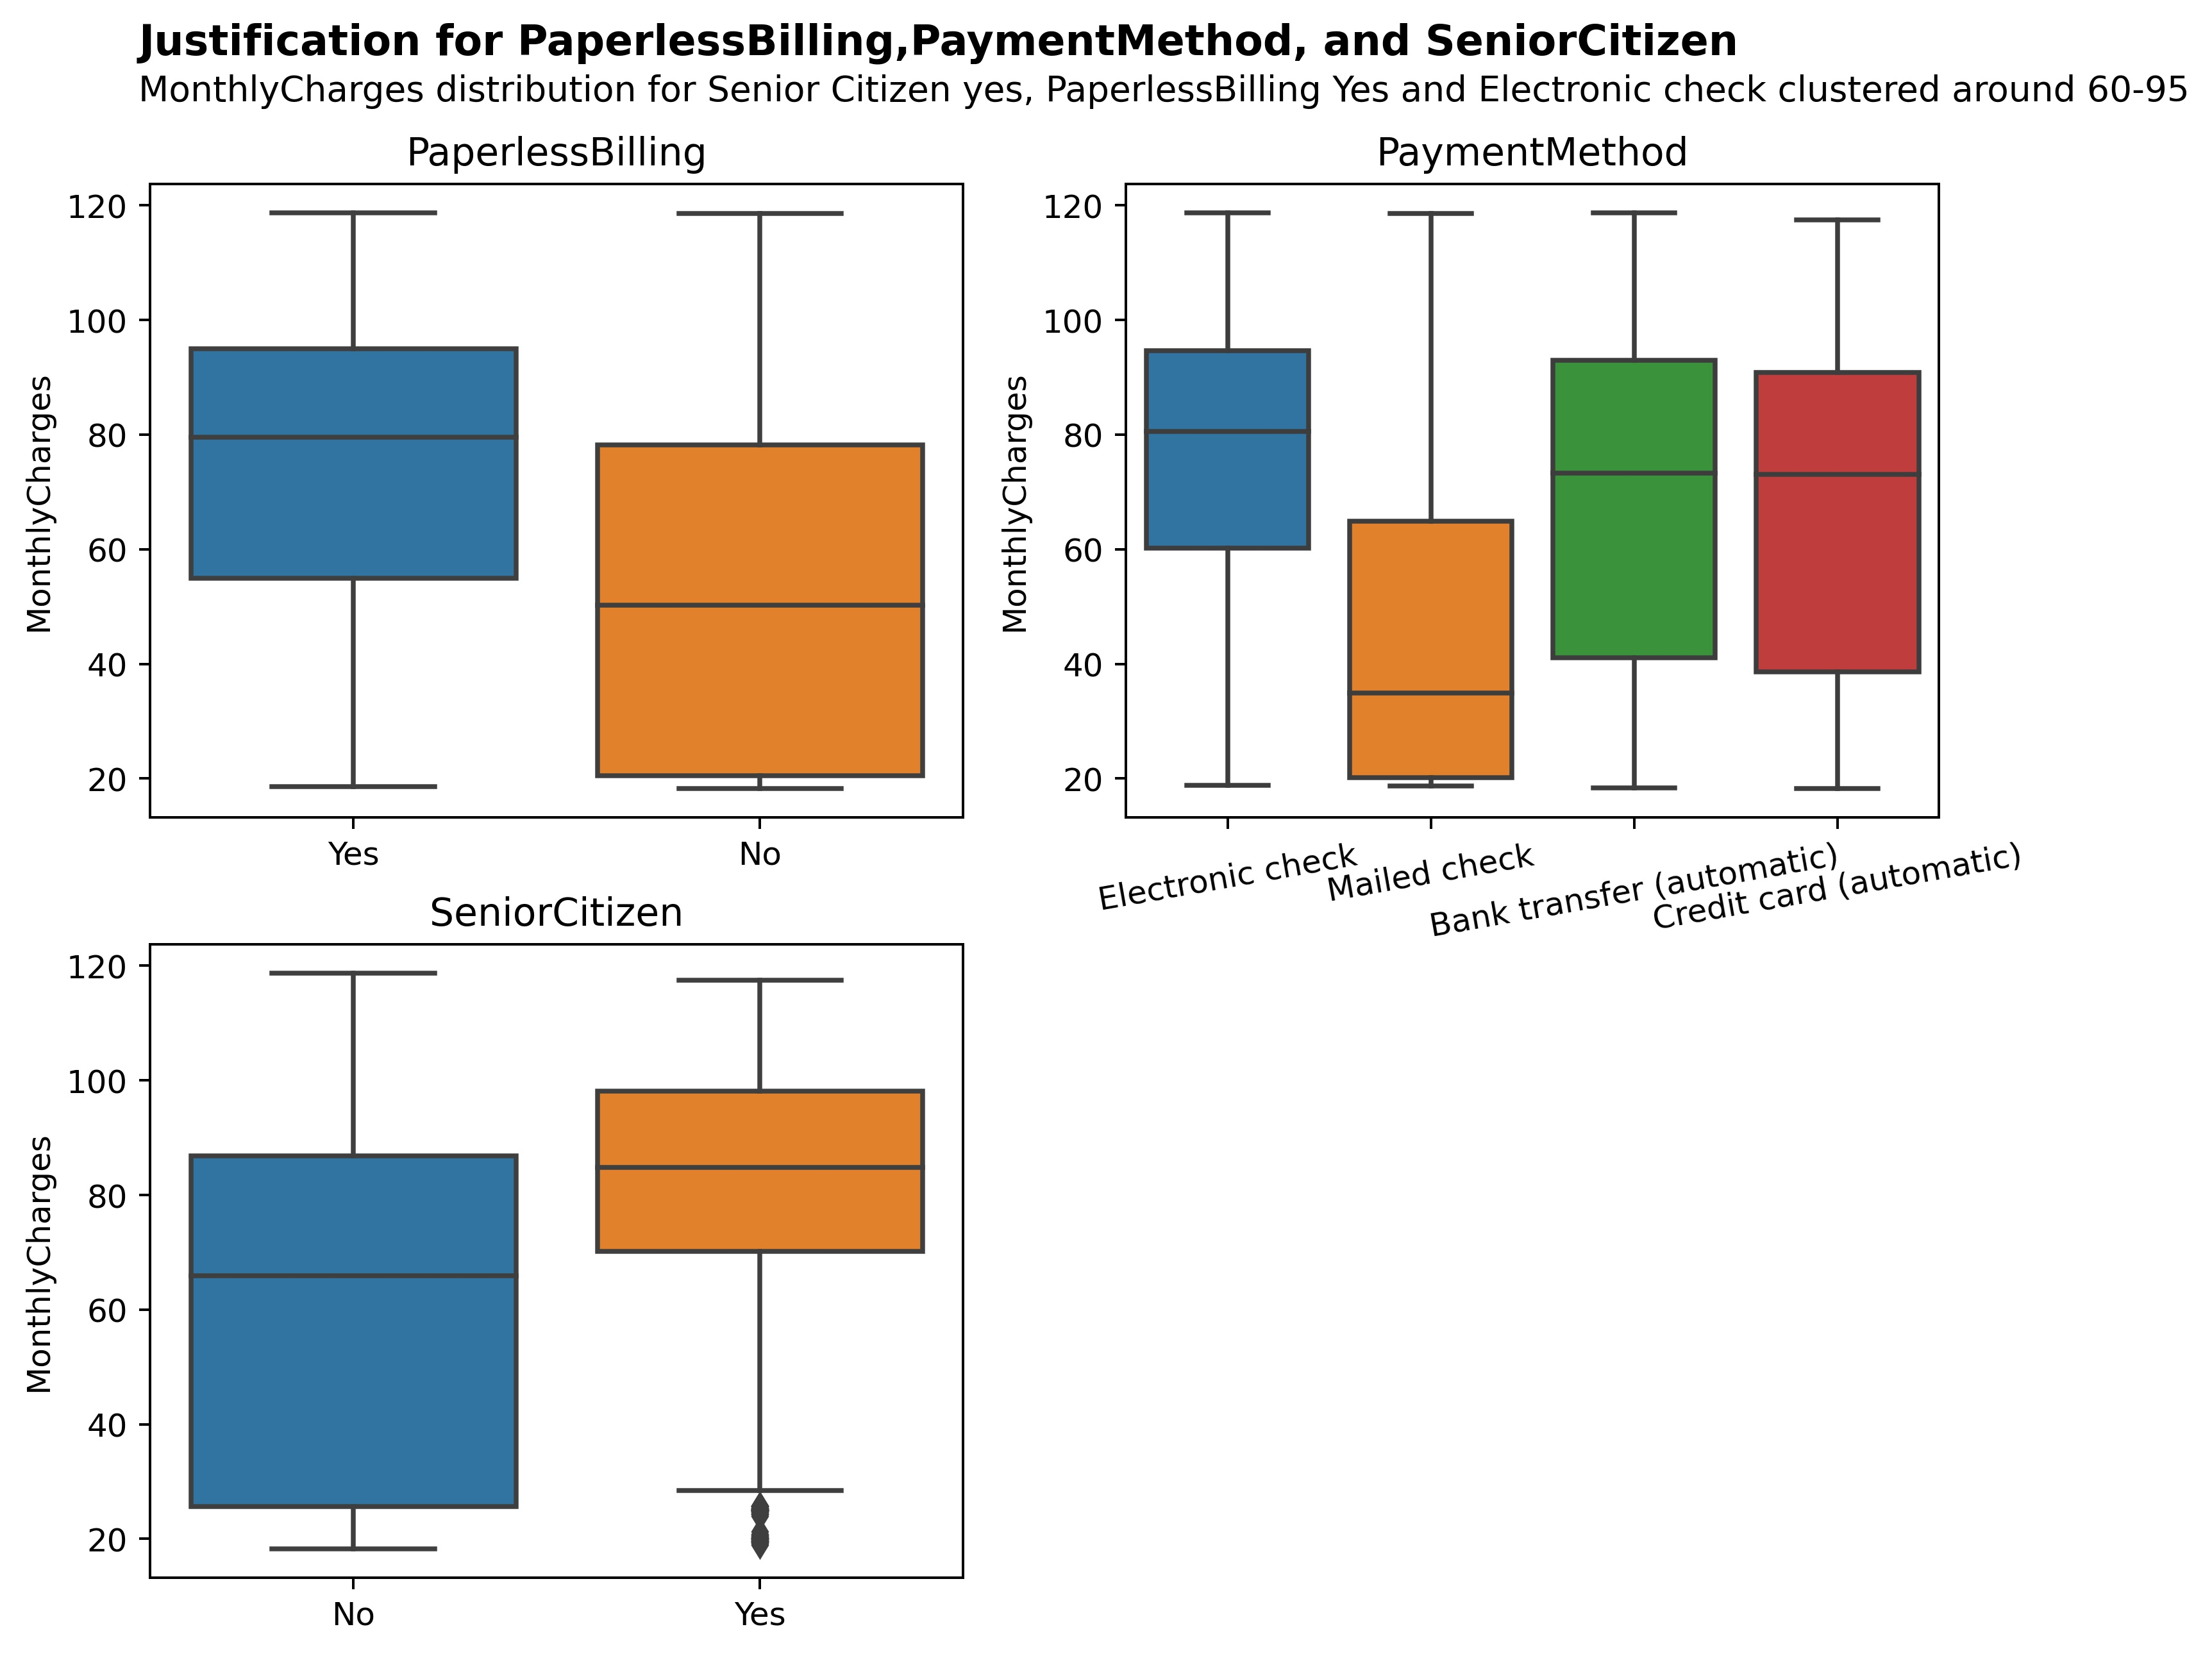
\includegraphics[width=0.9\linewidth]{figures/justify_sc}
	\caption{MonthlyCharges distribution for PaperlessBilling, SeniorCitizen and PaymentMethod}
	\label{fig:justify_sc}
\end{figure}

Another key takeaways from the preceding section is that many customers who join up for the streaming service choose to churn (more than other additional services such as OnlineSecurity, OnlineBackup, etc). Because the correlation matrix indicates that customers who use TV streaming services are more likely to use movies streaming services as well, these two variables will be combined to form a new variable, Streaming.

\begin{figure}[!htbp]
	\centering
	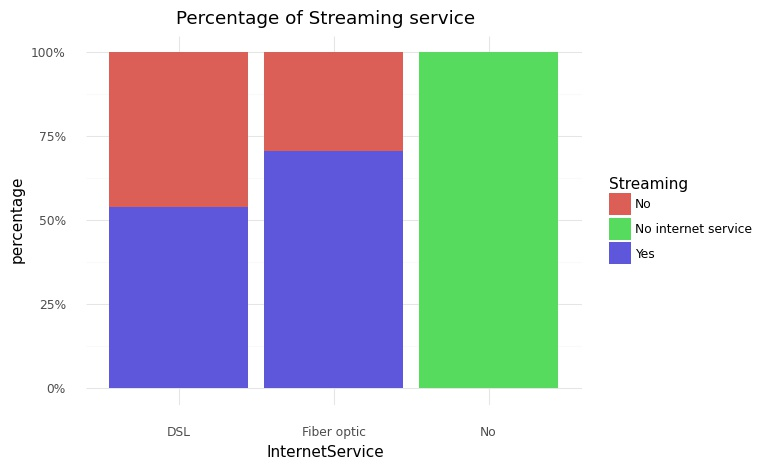
\includegraphics[width=0.8\linewidth]{figures/percentage_streaming}
	\caption{Percentage of streaming service enabled.}
	\label{fig:percentage_streaming}
\end{figure}

 Figure \ref{fig:percentage_streaming} shows that the vast majority of customers who use internet also sign up for the streaming service. It can be seen that roughly 70\% of Fiber optic users  subscribe for the streaming service. However, two important insights obtained from the previous section are both of these variables contribute to the churn decision. So in which variable does the main problem exist? Does it exist in the streaming service or the kind of the internet service itself, i.e Fiber optic?

\begin{figure}[!htbp]
	\centering
	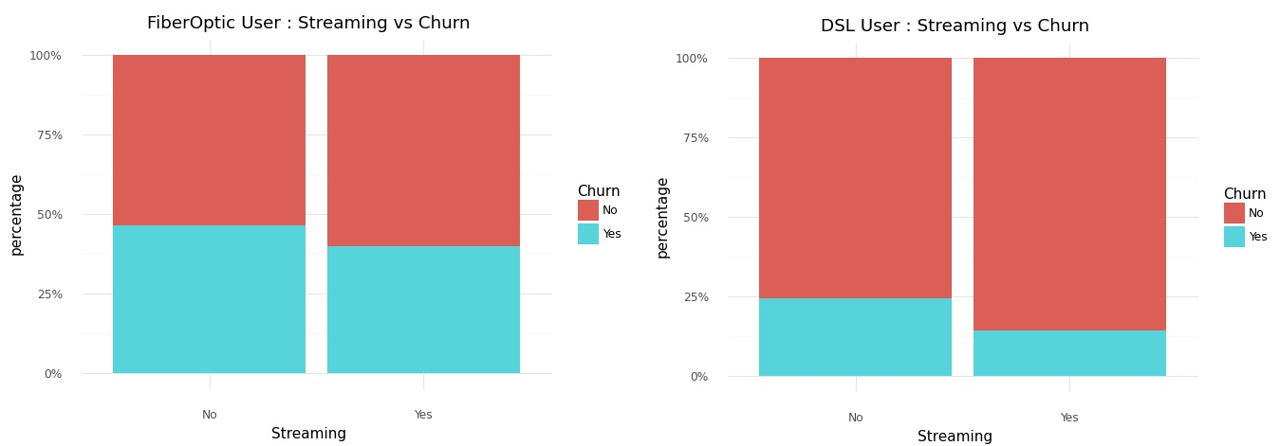
\includegraphics[width=1\linewidth]{figures/streaming_dsl_fiber}
	\caption{Percentage of lost customer in DSL and Fiber Optic.}
	\label{fig:streaming_dsl_fiber}
\end{figure}

Figure \ref{fig:streaming_dsl_fiber} appears as an answer to those questions. From Figure \ref{fig:streaming_dsl_fiber} it is evident that the customers who do not subscribe for any Streaming services actually have slightly higher probability to churn in both DSL and Fiber optic services. Moreover, the Churn probability for Fiber optic users almost two times higher than DSL users. Both of these findings indicate that the major issue is the Fiber Optic service itself.

\begin{figure}[!htbp]
	\centering
	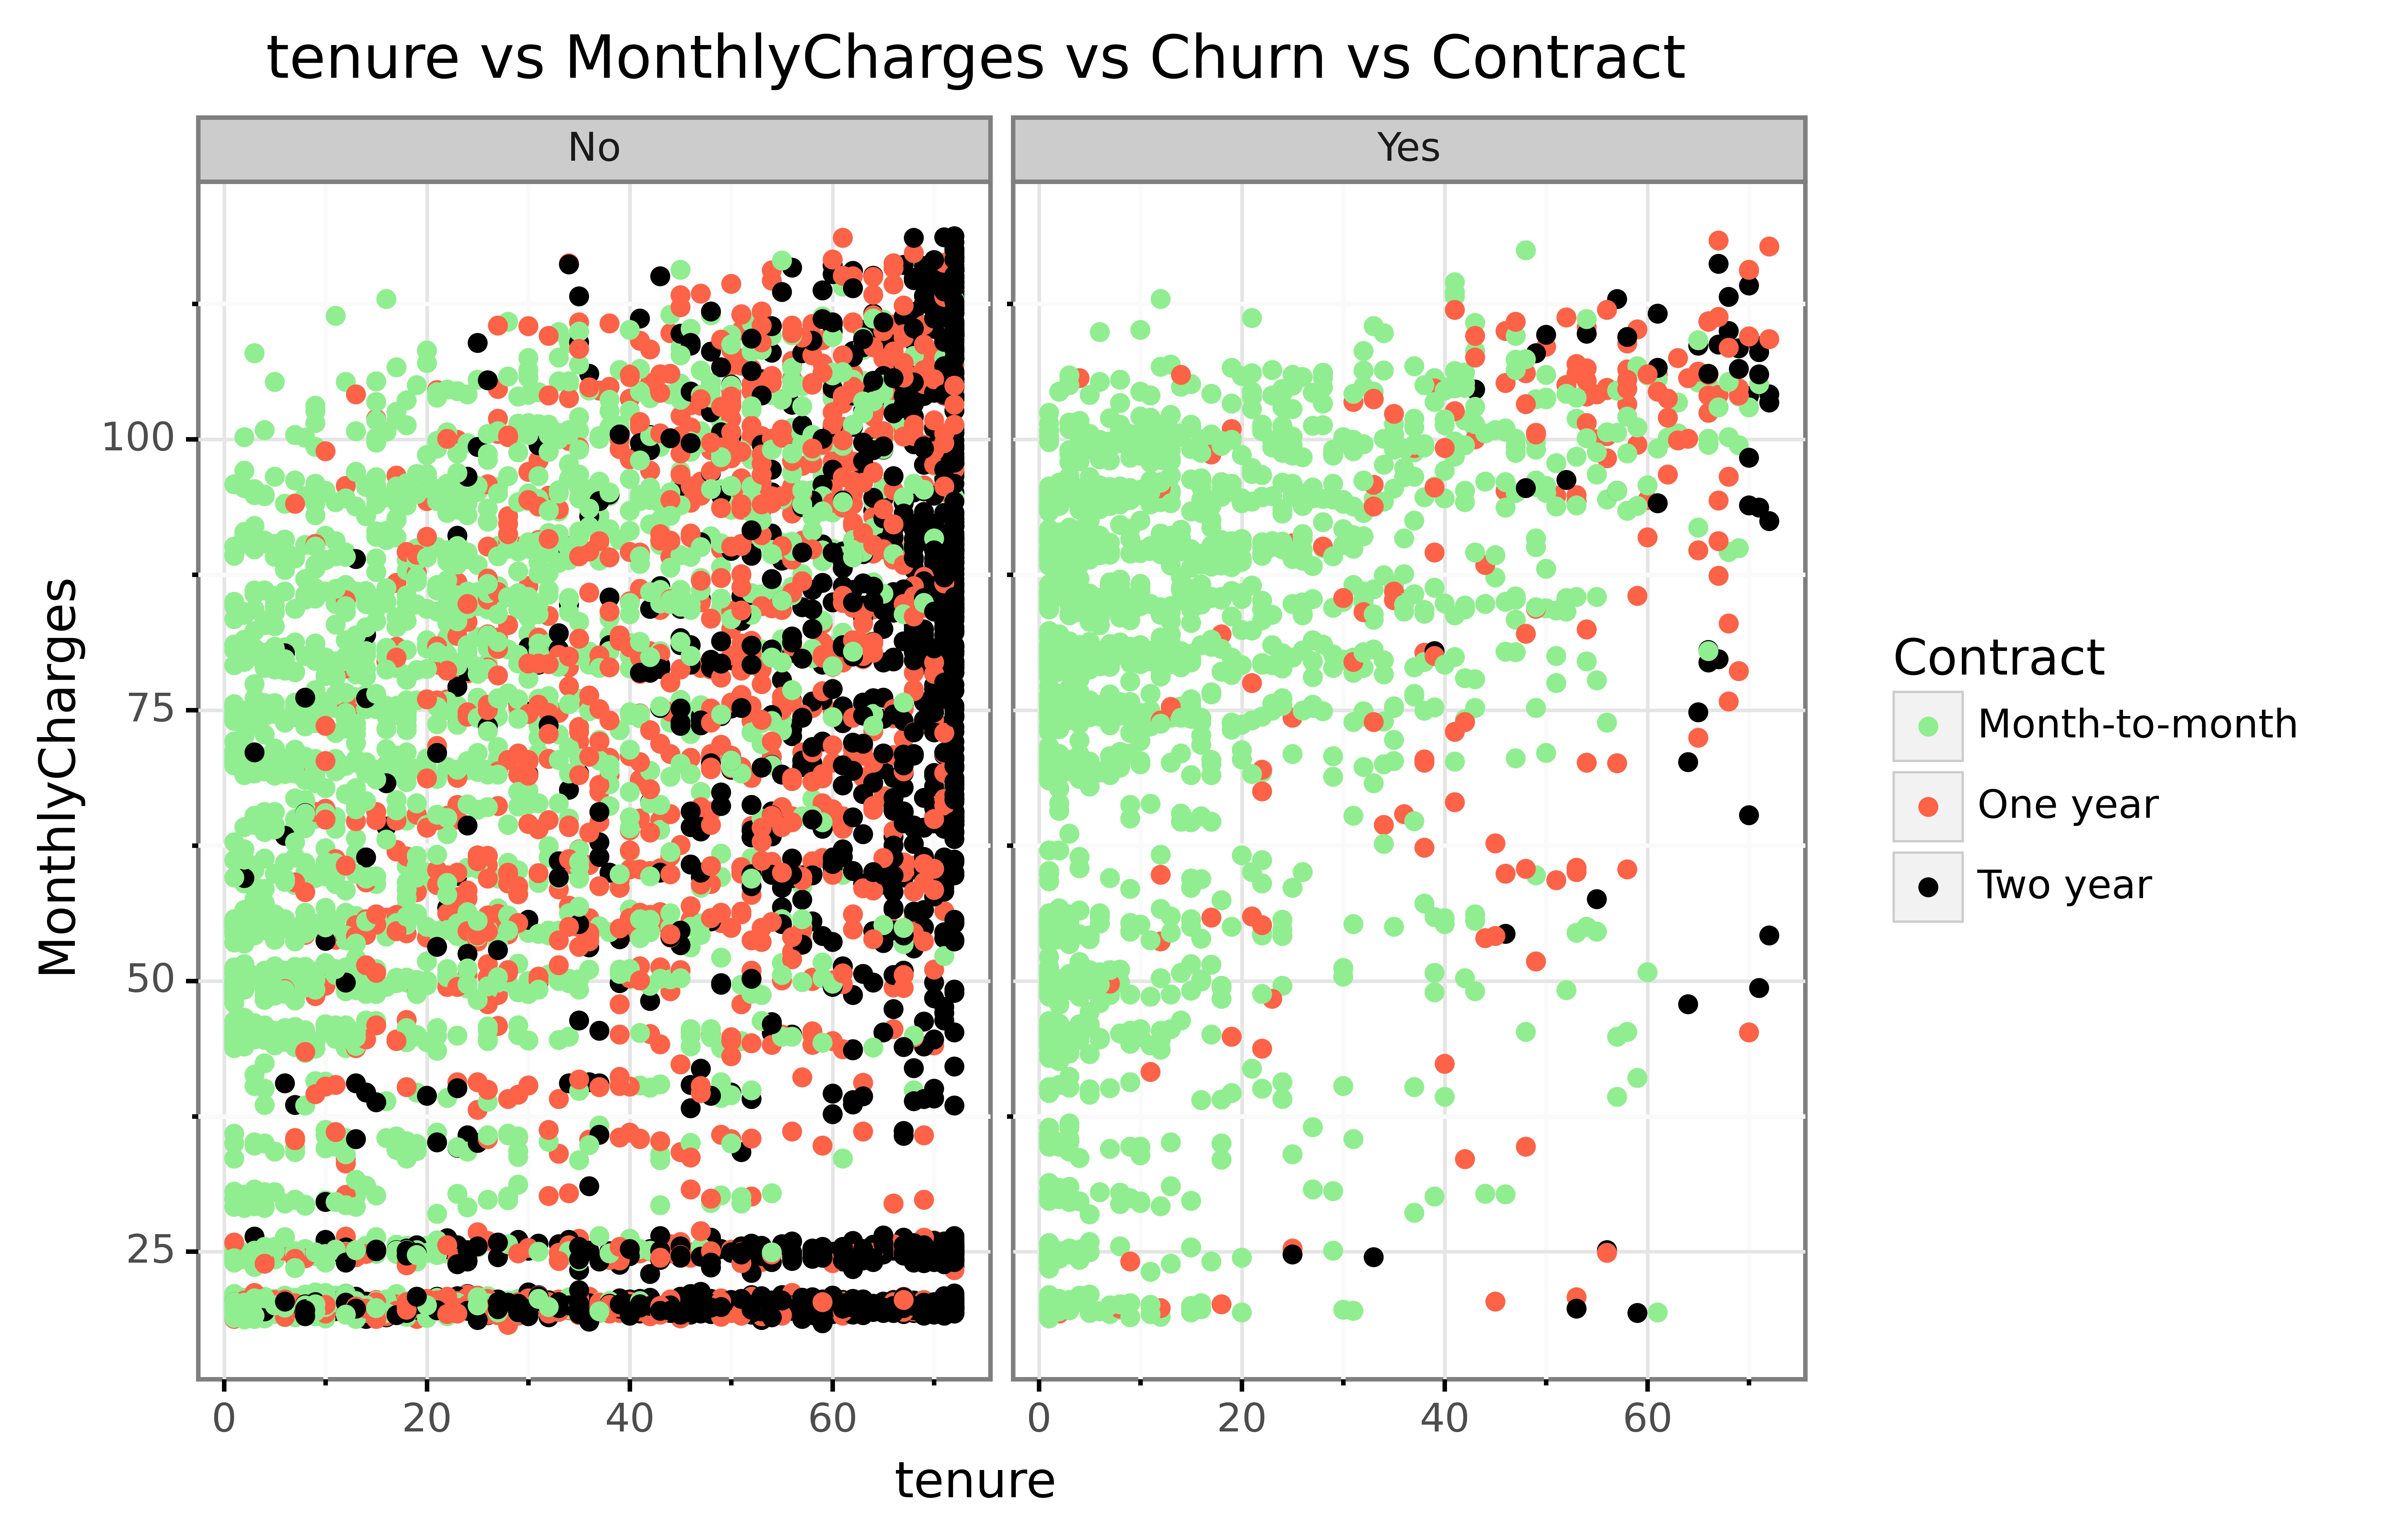
\includegraphics[width=0.9\linewidth]{figures/tenurechurn}
	\caption{Scatter plot of tenure,MonthlyCharges, Churn (Yes and No), and Contract.}
	\label{fig:tenure_churn}
\end{figure}
In addition to InternetService, tenure is another significant factor in this dataset. Figure \ref{fig:tenure_churn} shows that practically almost every value of MonthlyCharges has customers who churn in their first 6 months. This suggests that the majority of new telecom customers may have negative beginning experiences. Another finding is as tenure increases the contract also increases from monthly becomes yearly. That's why in the small tenure period, mostly the contracts are monthly and customers with that contract are more likely to churn than those who have yearly contract.  This finding is actually quite reasonable because monthly contract customers are frequently new and still not satisfied enough with the service quality and unsure whether they will remain loyal to the company. That's why one also can see that as the period of contract increases the churn probability decreases.
 
	\section{Conclusion}
From all the results above it can be concluded that :
\begin{enumerate}
	\item In the last month, the company lost 1869 its customers, representing a churn rate of approximately 27\%. The main causes of customer churn are poor quality Fiber optic services and negative first-time customer experiences. As a result, nearly 42\% of Fiber optic users chose to churn in the last month, and more than 55\% of new customers (only subscribed for less than 4 months) chose to churn as well.
	\item Because the vast majority of customers (44\%) actually sign up for fiber optic service and pay such high monthly fees (around 70-120 dollars), the company should focus more on improving the quality in order to reduce its significant revenue loss. They should also improve the experience of their new customers and target those who are young or middle-aged, have a partner or dependents, as they are less likely to churn.
\end{enumerate}
	
	
	
	
	%If you came here because you want your references in a new page, uncomment the following line
	
	%\clearpage % If you want the references in a separate page
	\newpage
	\bibliography{bibliography}
	\addcontentsline{toc}{section}{References}
	
	\clearpage % If you want the appendix in a separate page
%	\appendix
%	\input{sections/appendix}
	
\end{document}